\section{Data to Monte Carlo comparisons at $\sqrt{s}=900$ GeV in
  Minimum Bias events}
\label{sc:DataVsMCMB900}

In this section we present the comparison of several calorimeter-based
distributions in data with {\sc pythia} Mininimum Bias Monte Carlo simulation. All distributions
shown in this section are required to pass the event selections
described in Sec.4. The Monte Carlo distributions shown in this section
are normalized so that the total number of events in Monte Carlo sample
mathces the number of events observed in data.


\subsection{Basic $\etmiss$-related distributions.}
\begin{figure}[h!]
 \centering
 \begin{tabular}{ll}
  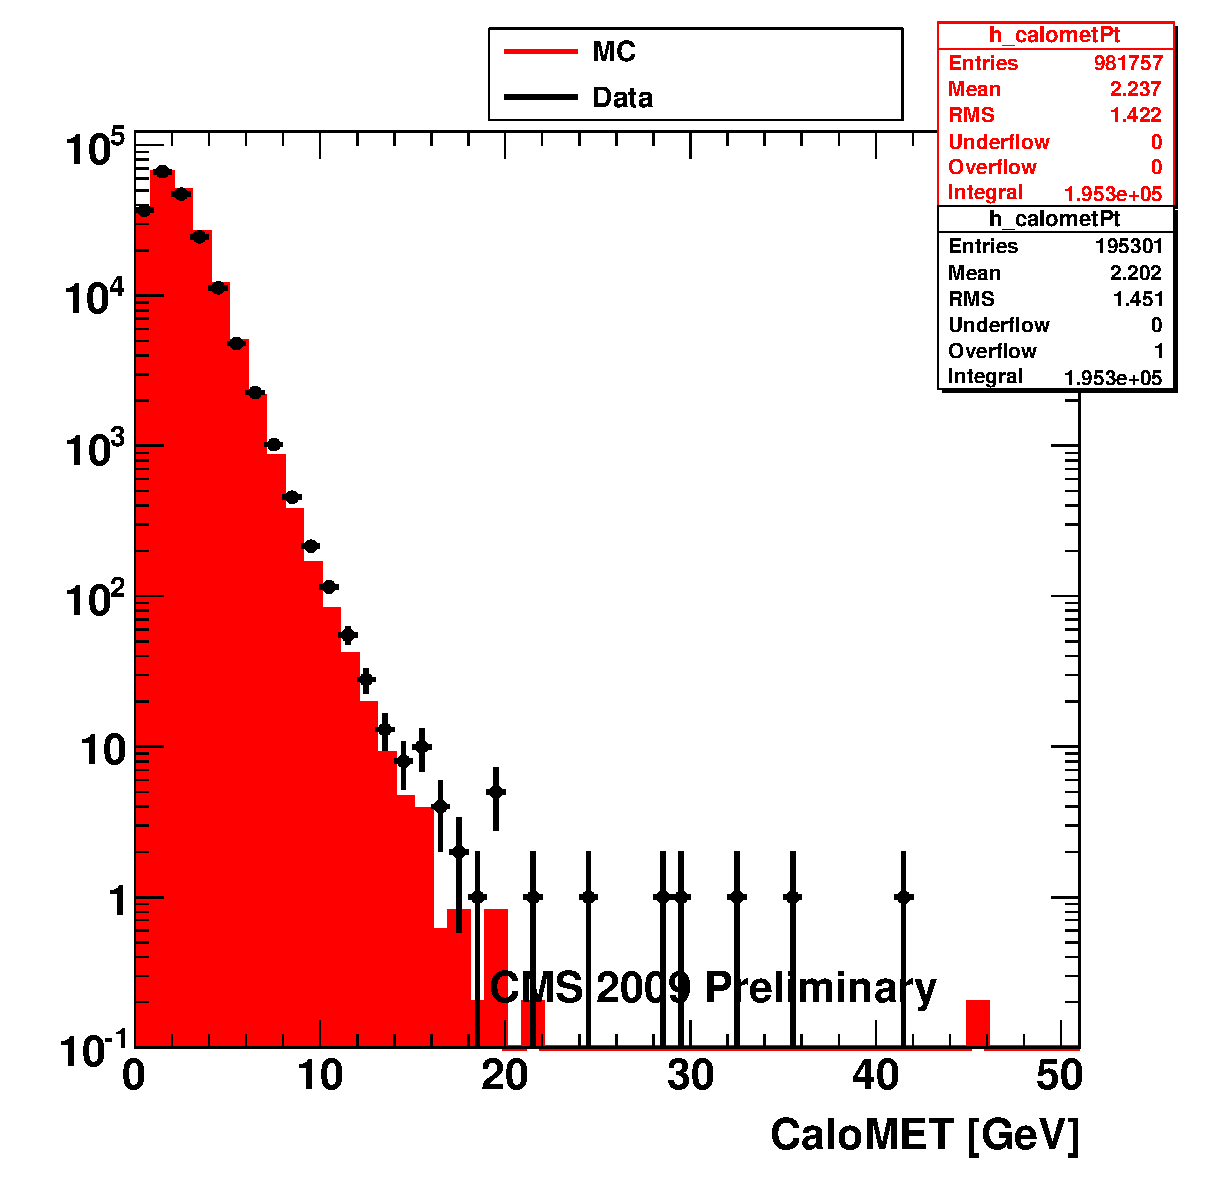
\includegraphics[width=0.40\textwidth]{plots_DataVsMC_MB_900GeV/h_calometPt.eps} &
  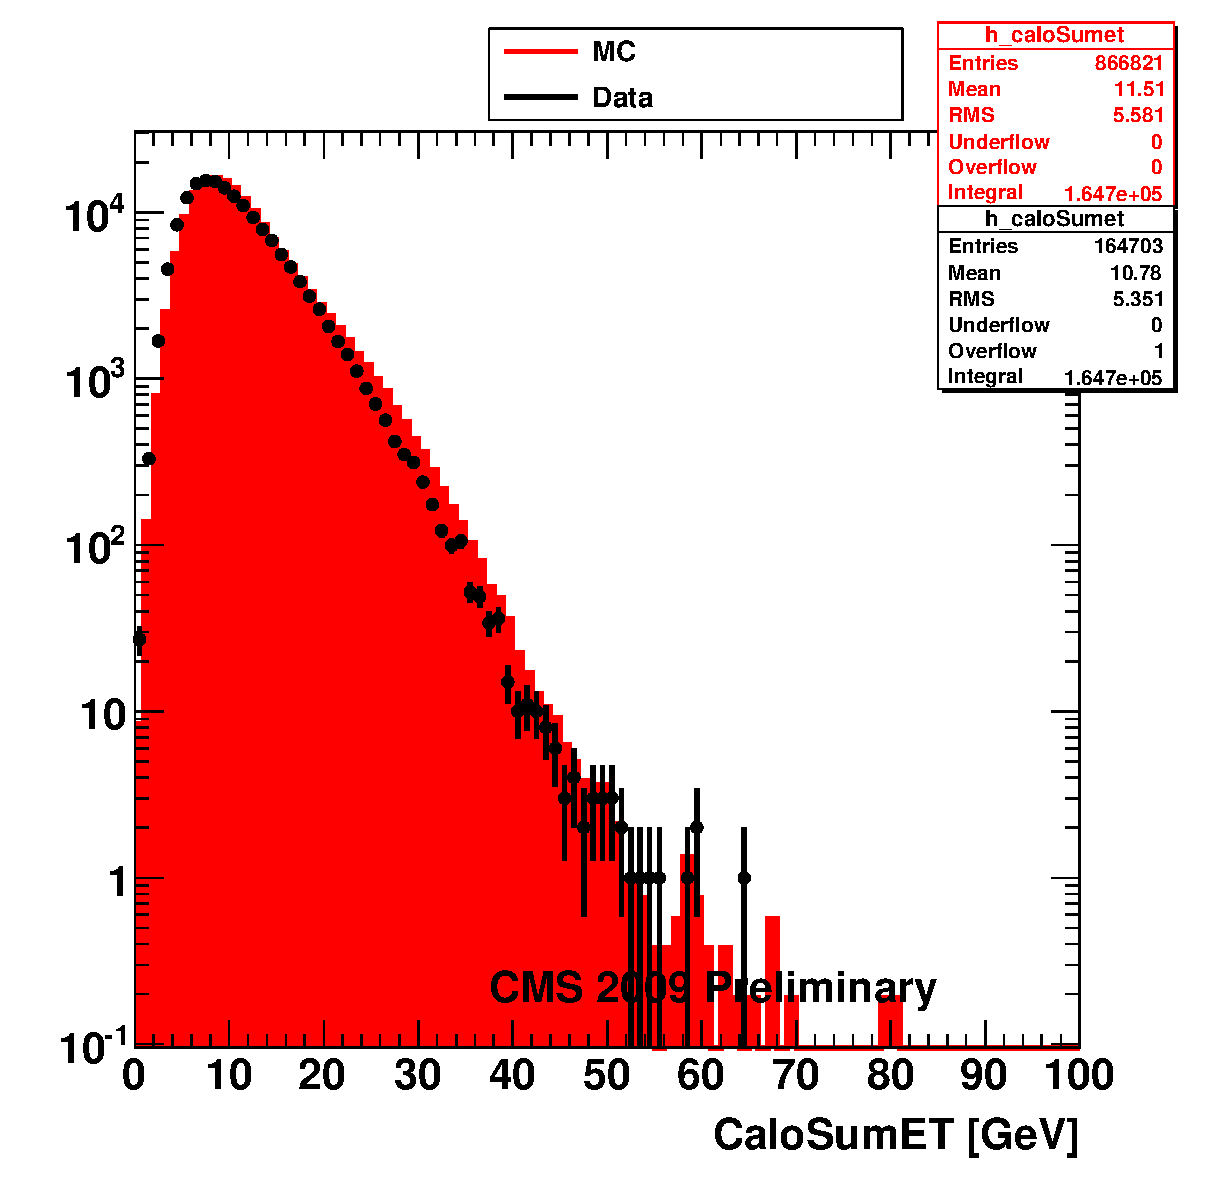
\includegraphics[width=0.40\textwidth]{plots_DataVsMC_MB_900GeV/h_caloSumet.eps} \\
 \end{tabular}
 \caption{$\etmiss$ and SumET distributions in 900 GeV data compared
   with Monte Carlo simulation.
          \label{fig:DataVsMC_MB_900_1}}
\end{figure}

\begin{figure}[h!]
 \centering
 \begin{tabular}{ll}
  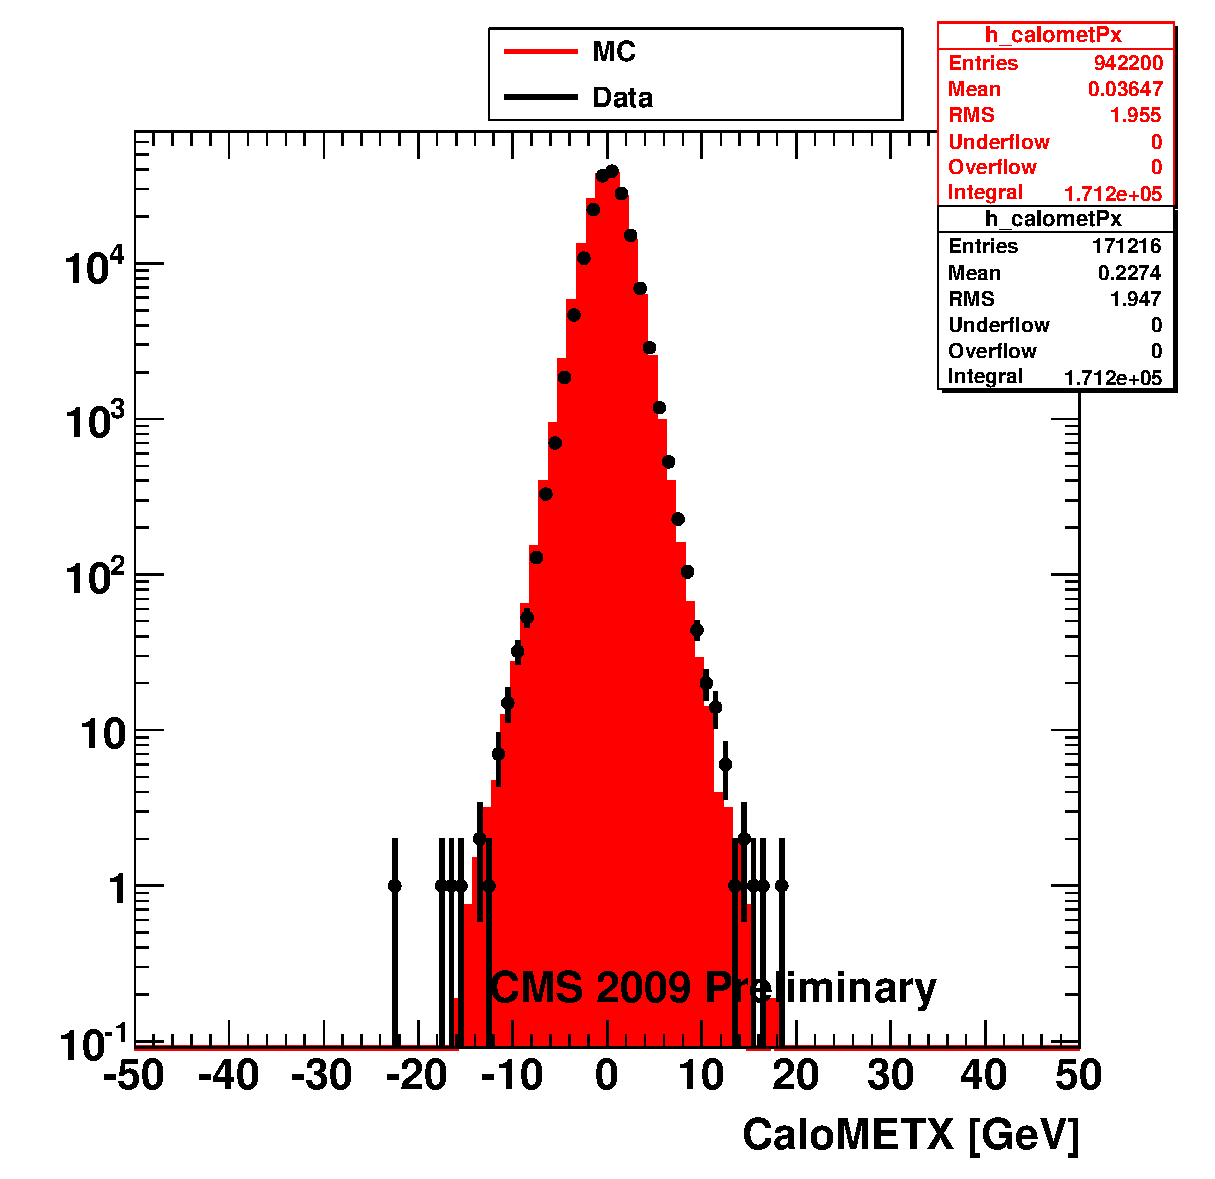
\includegraphics[width=0.40\textwidth]{plots_DataVsMC_MB_900GeV/h_calometPx.eps} &
  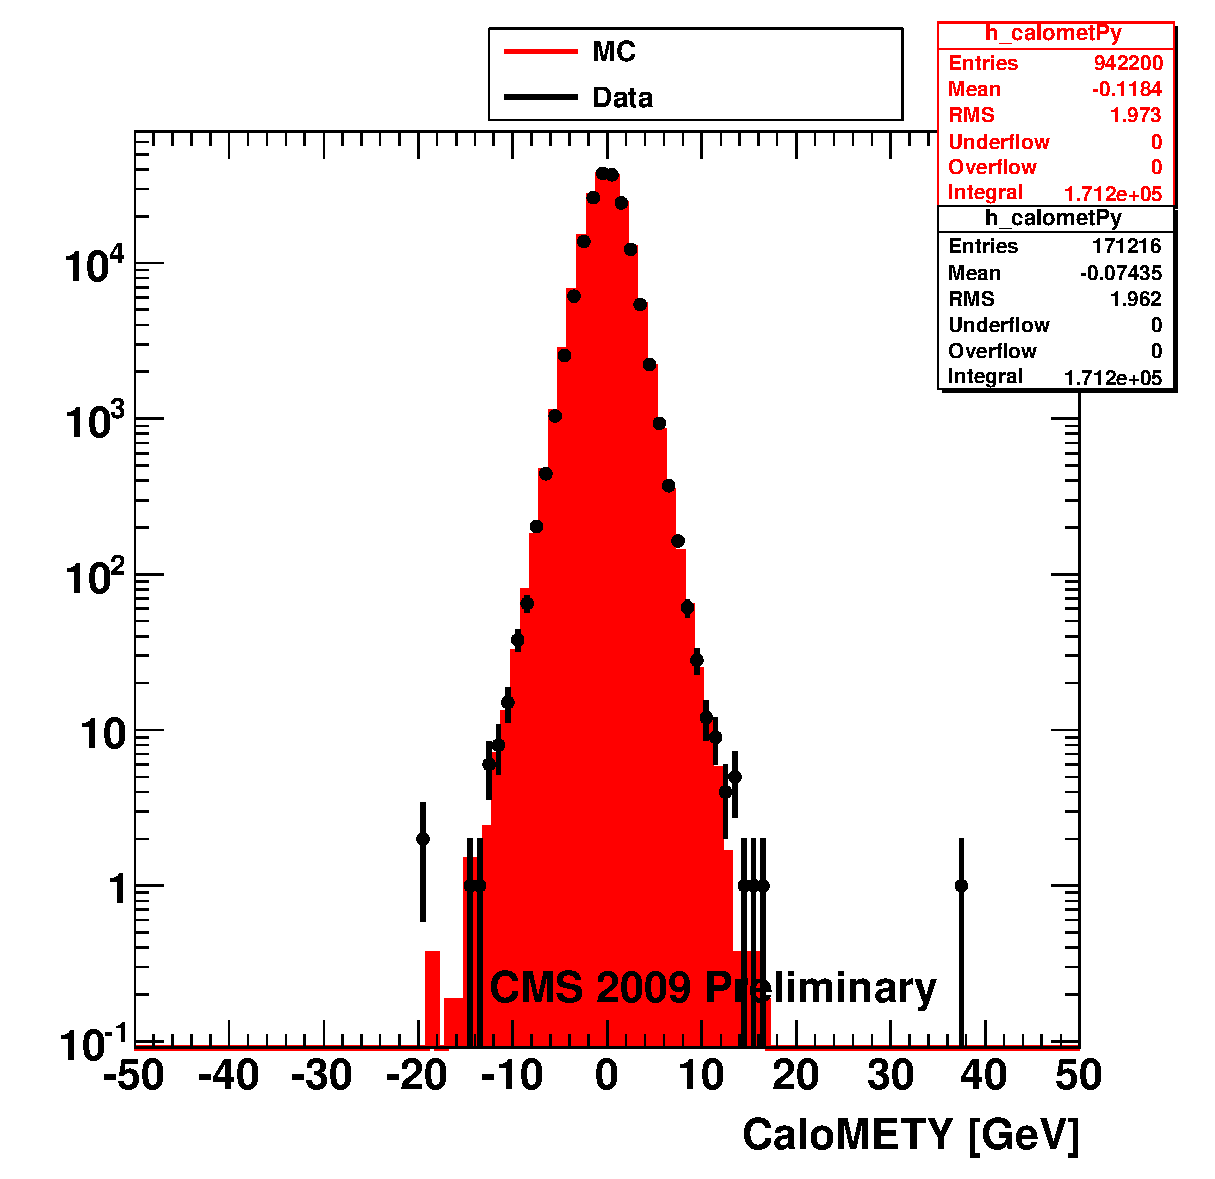
\includegraphics[width=0.40\textwidth]{plots_DataVsMC_MB_900GeV/h_calometPy.eps} \\
 \end{tabular}
 \caption{$\exmiss$ and $\eymiss$ distributions in 900 GeV data compared
   with Monte Carlo simulation.
          \label{fig:DataVsMC_MB_900_2}}
\end{figure}

\begin{figure}[h!]
 \centering
 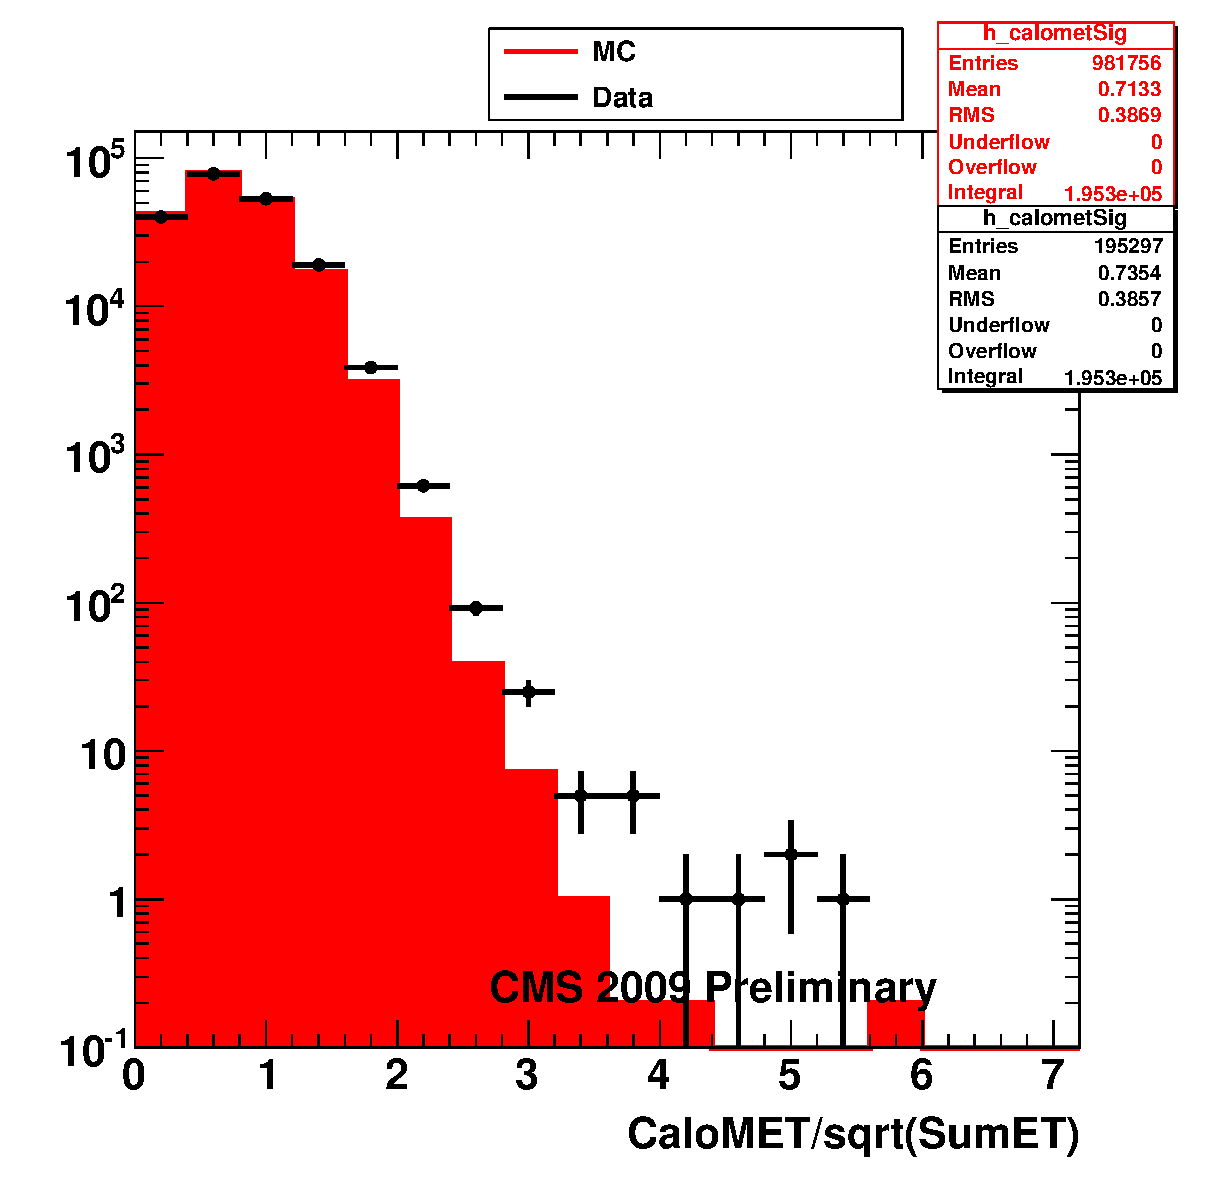
\includegraphics[width=0.40\textwidth]{plots_DataVsMC_MB_900GeV/h_calometSig.eps}
\caption{$\etmiss^{Sig}=\etmiss/\sqrt{SumET}$ distributions in 900 GeV data compared
   with Monte Carlo simulation.
          \label{fig:DataVsMC_MB_900_3}}
\end{figure}

\begin{figure}[h!]
 \centering
 \begin{tabular}{ll}
  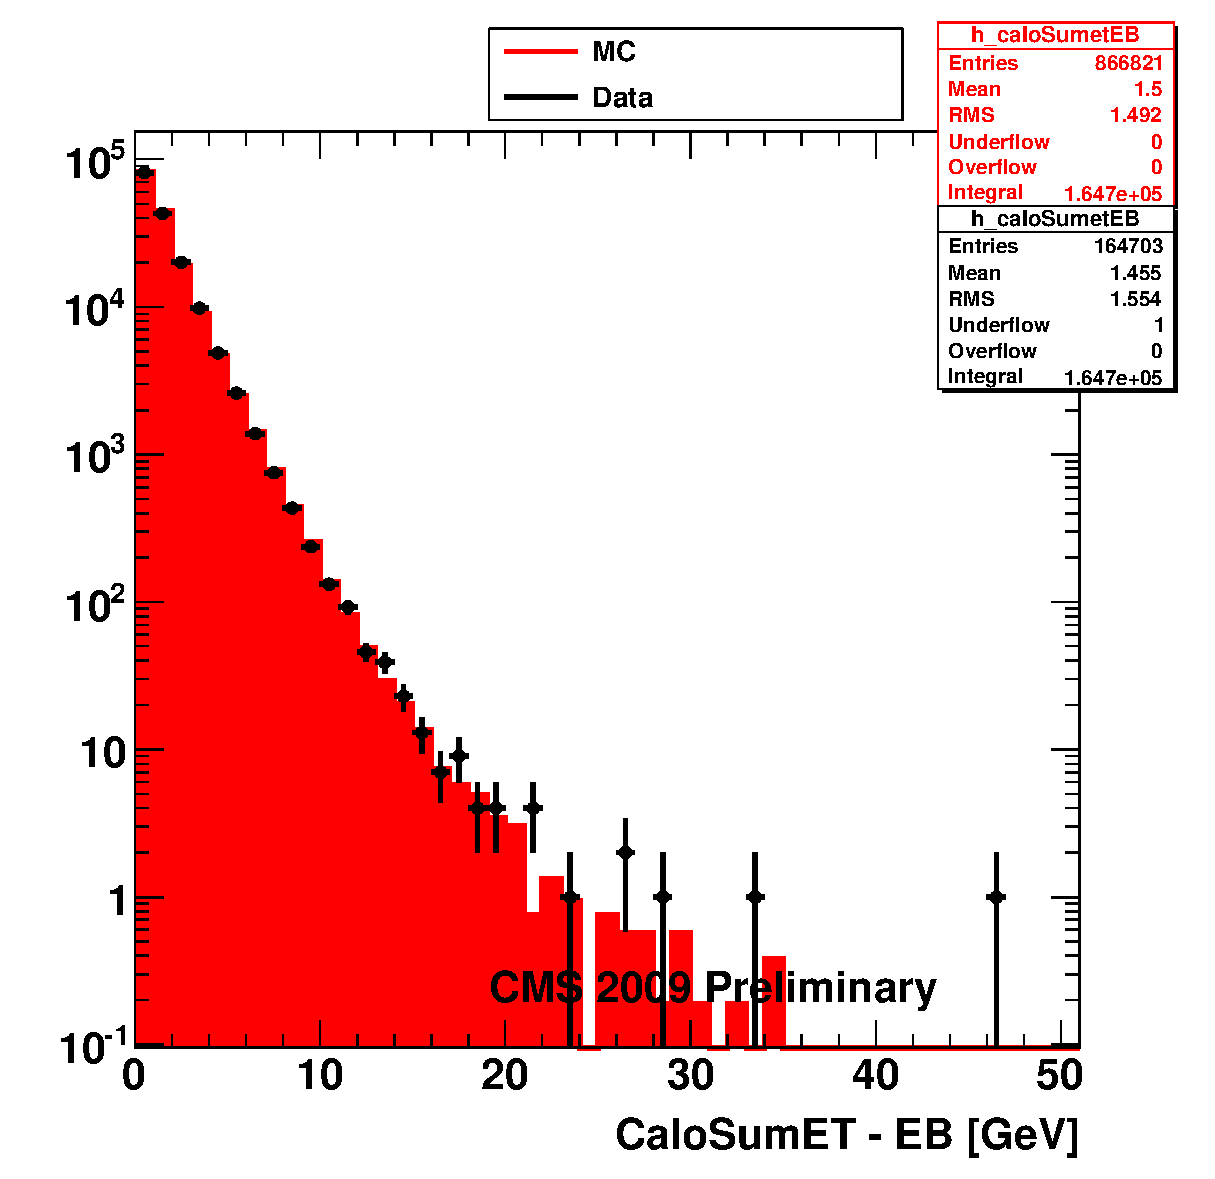
\includegraphics[width=0.40\textwidth]{plots_DataVsMC_MB_900GeV/h_caloSumetEB.eps} &
  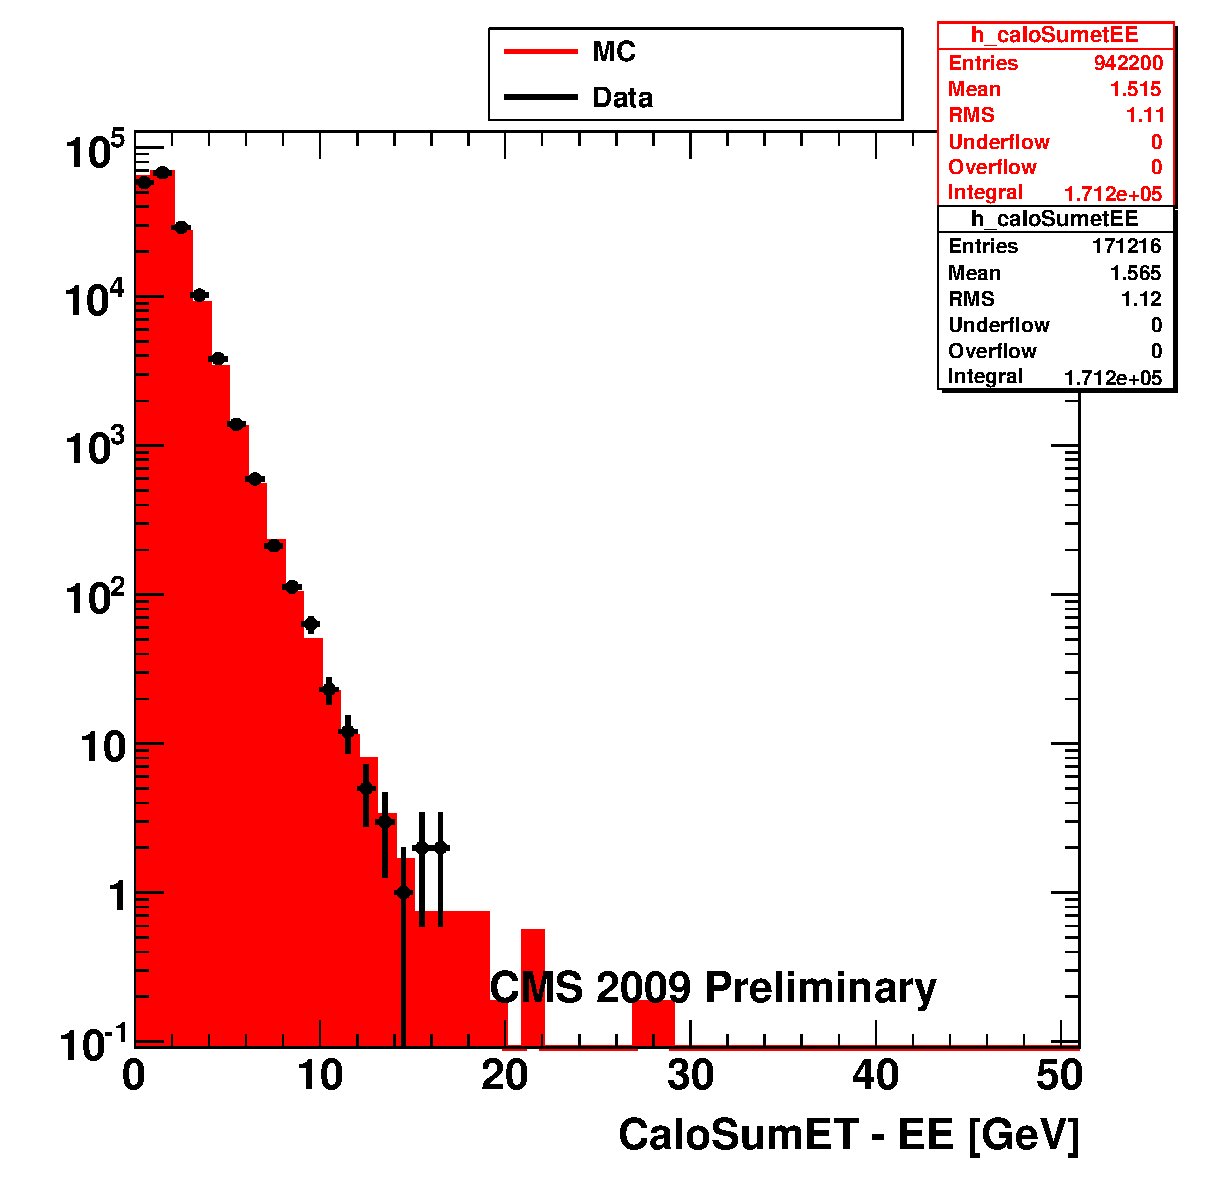
\includegraphics[width=0.40\textwidth]{plots_DataVsMC_MB_900GeV/h_caloSumetEE.eps} \\
 \end{tabular}
 \caption{SumET in ECAL barrel and endcap in 900 GeV data compared
   with Monte Carlo simulation.
          \label{fig:DataVsMC_MB_900_4}}
\end{figure}

\begin{figure}[h!]
 \centering
 \begin{tabular}{ll}
  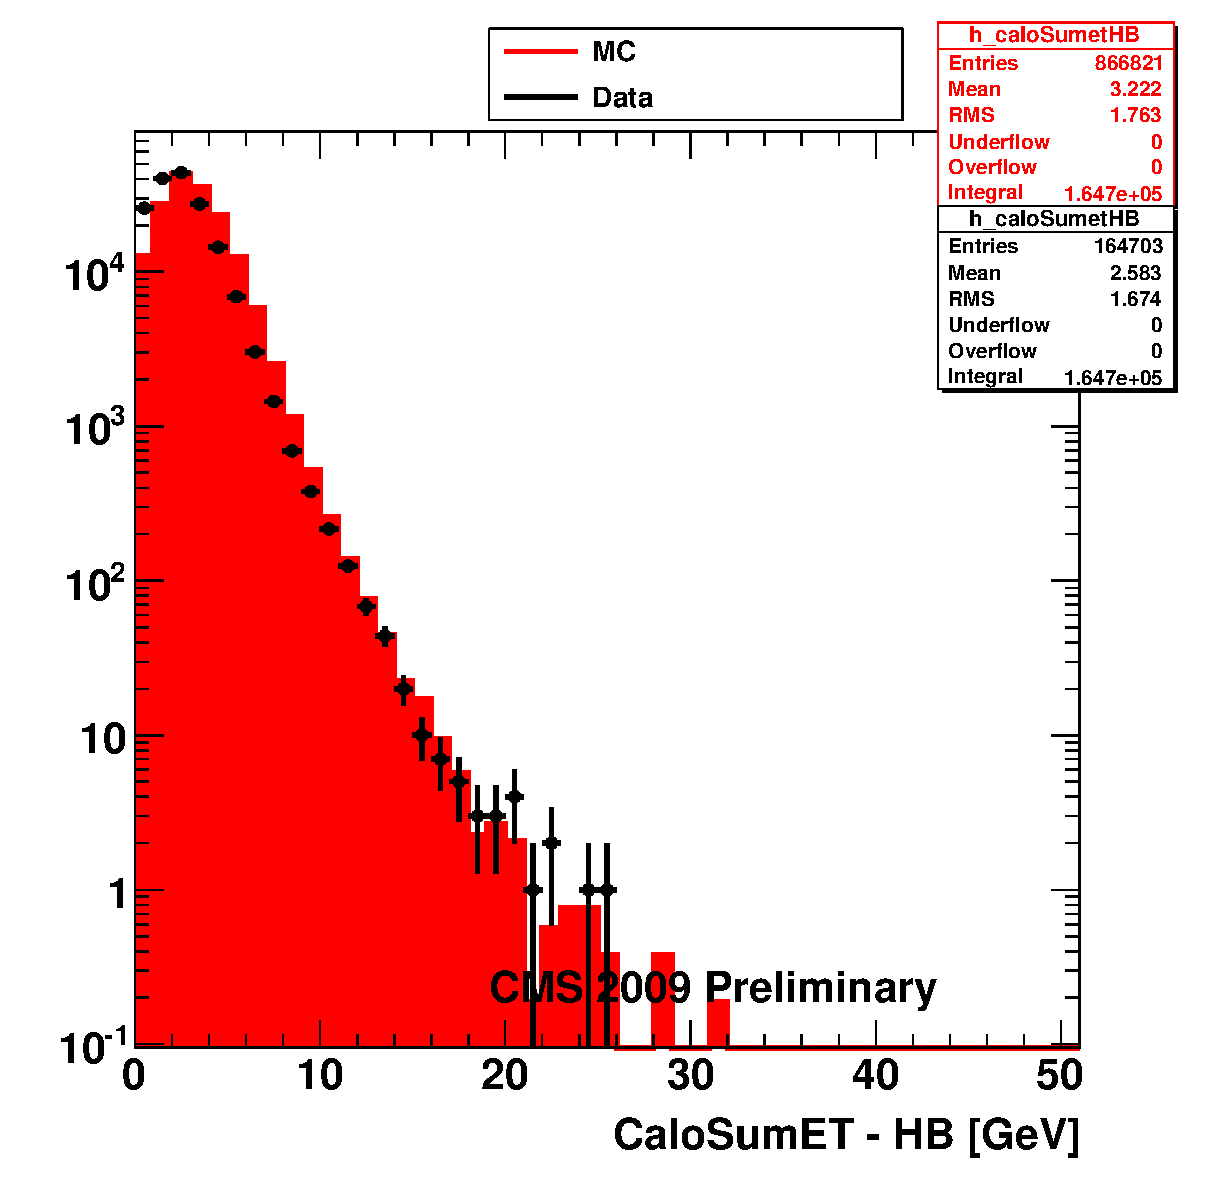
\includegraphics[width=0.40\textwidth]{plots_DataVsMC_MB_900GeV/h_caloSumetHB.eps} &
  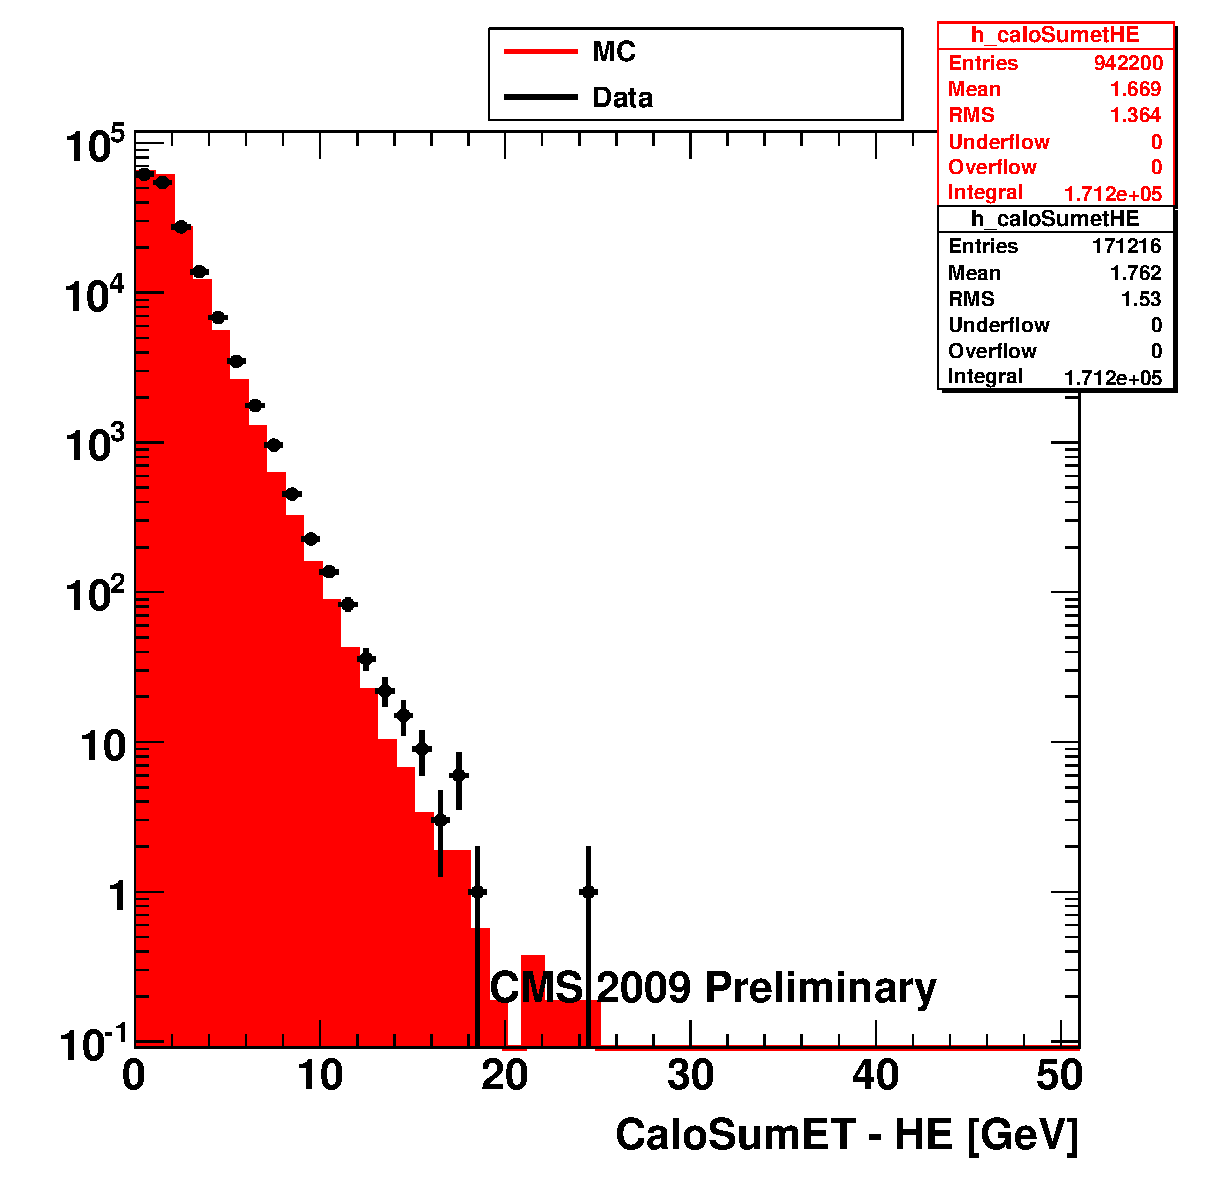
\includegraphics[width=0.40\textwidth]{plots_DataVsMC_MB_900GeV/h_caloSumetHE.eps} \\
 \end{tabular}
 \caption{SumET in HCAL barrel and endcap in 900 GeV data compared
   with Monte Carlo simulation.
          \label{fig:DataVsMC_MB_900_5}}
\end{figure}

\begin{figure}[h!]
 \centering
 \begin{tabular}{ll}
  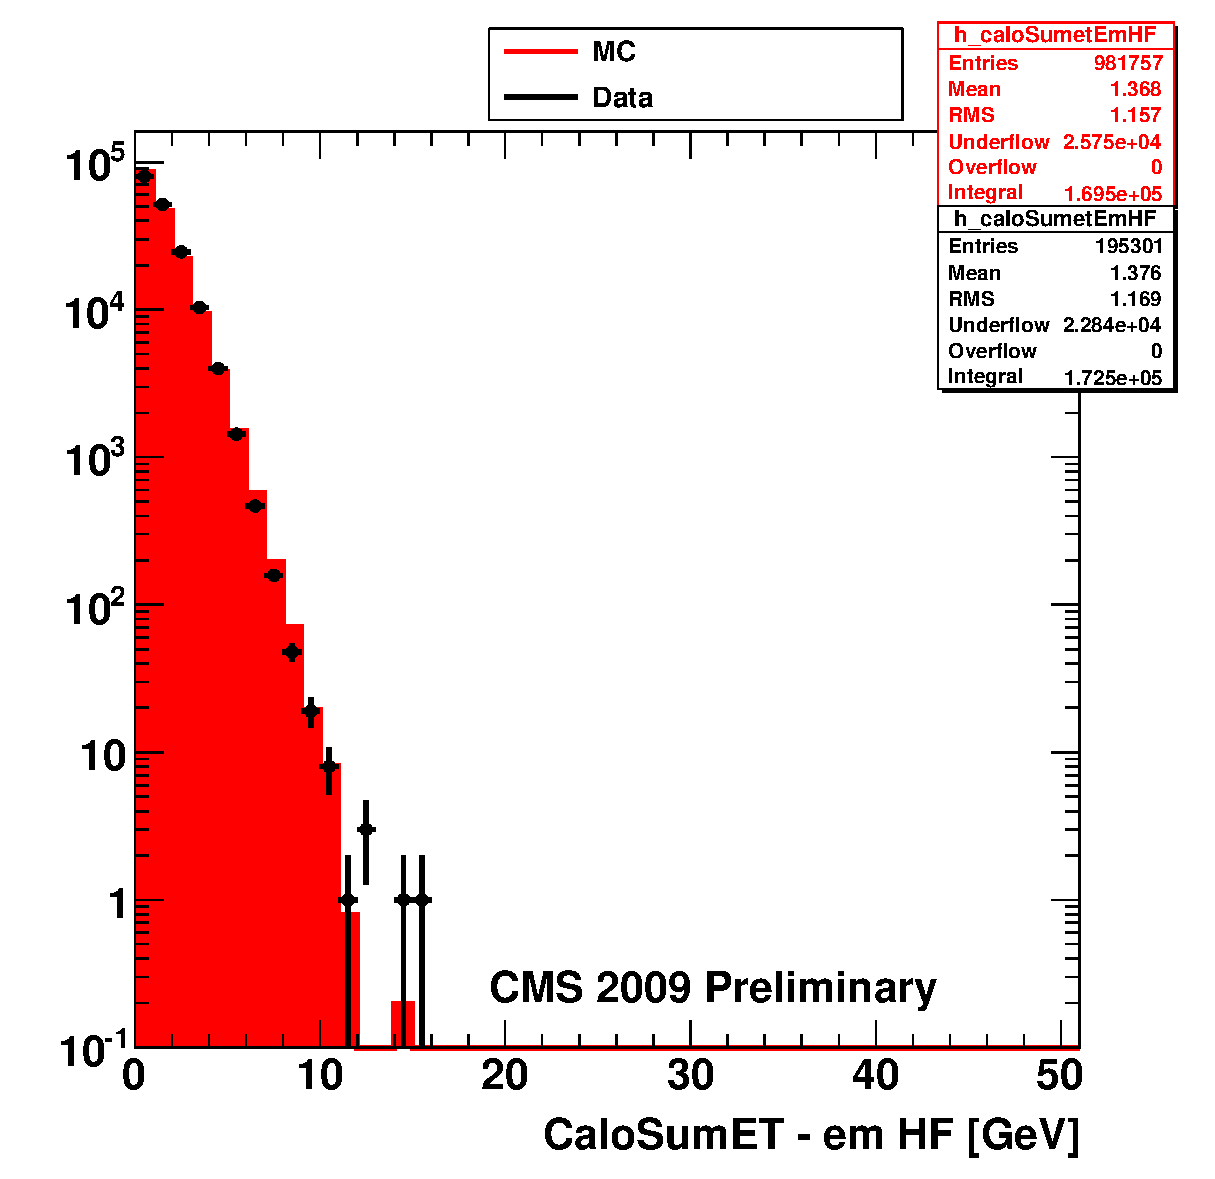
\includegraphics[width=0.40\textwidth]{plots_DataVsMC_MB_900GeV/h_caloSumetEmHF.eps} &
  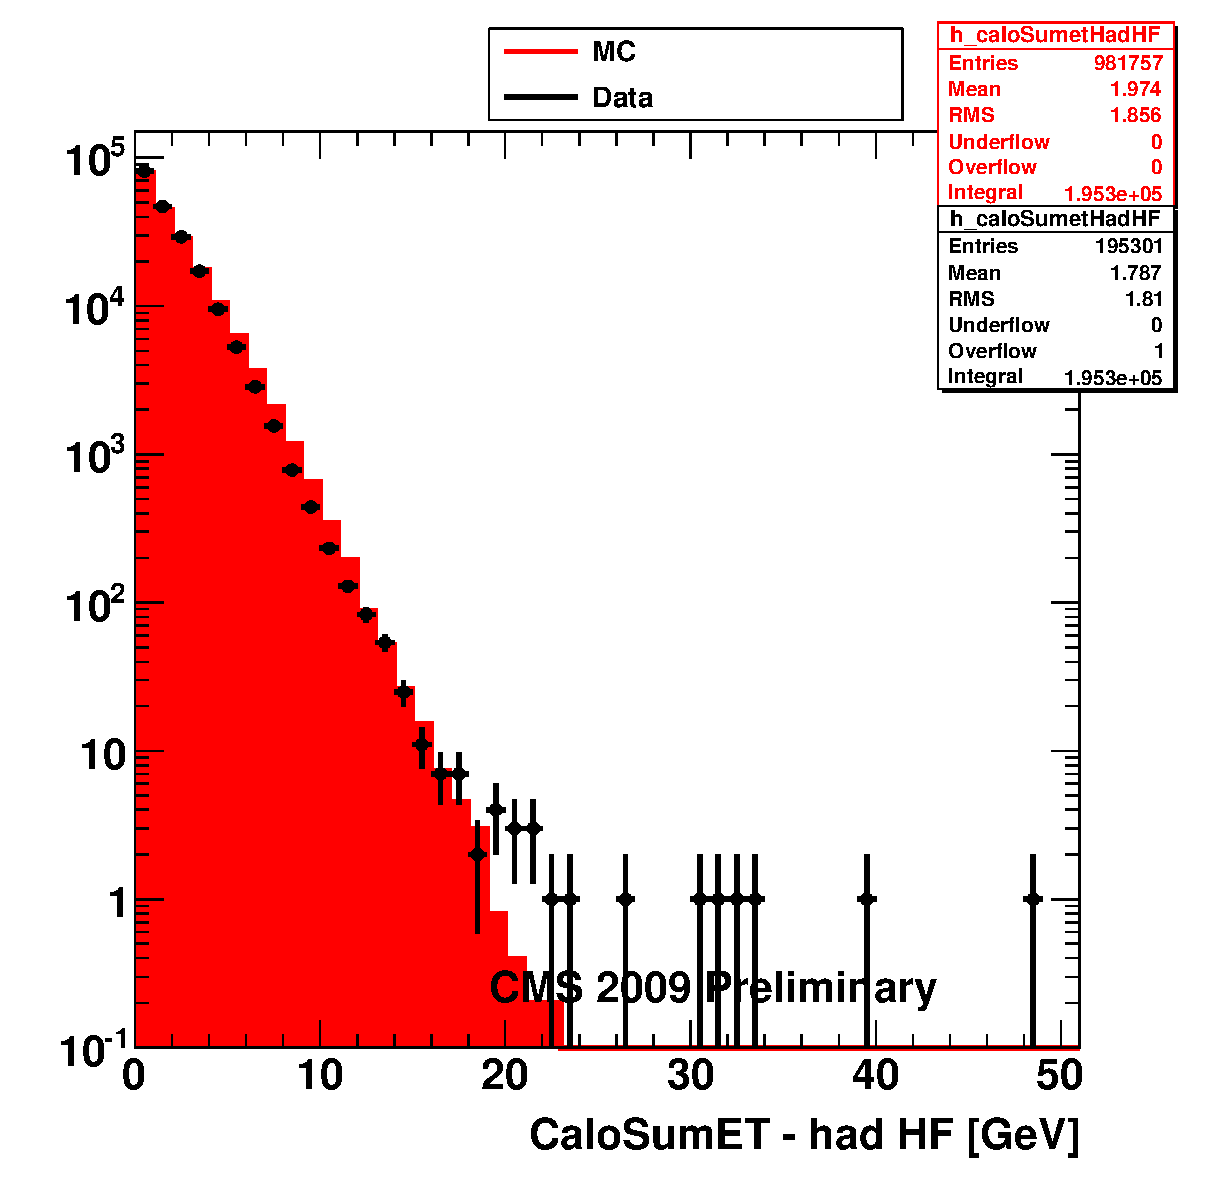
\includegraphics[width=0.40\textwidth]{plots_DataVsMC_MB_900GeV/h_caloSumetHadHF.eps} \\
 \end{tabular}
 \caption{SumET in HF in electromagnetic and hadronic parts in 900 GeV data compared
   with Monte Carlo simulation.
          \label{fig:DataVsMC_MB_900_6}}
\end{figure}

\clearpage

\subsection{$\etmiss$ resolution.}

\begin{figure}[h!]
 \centering
 \begin{tabular}{ll}
  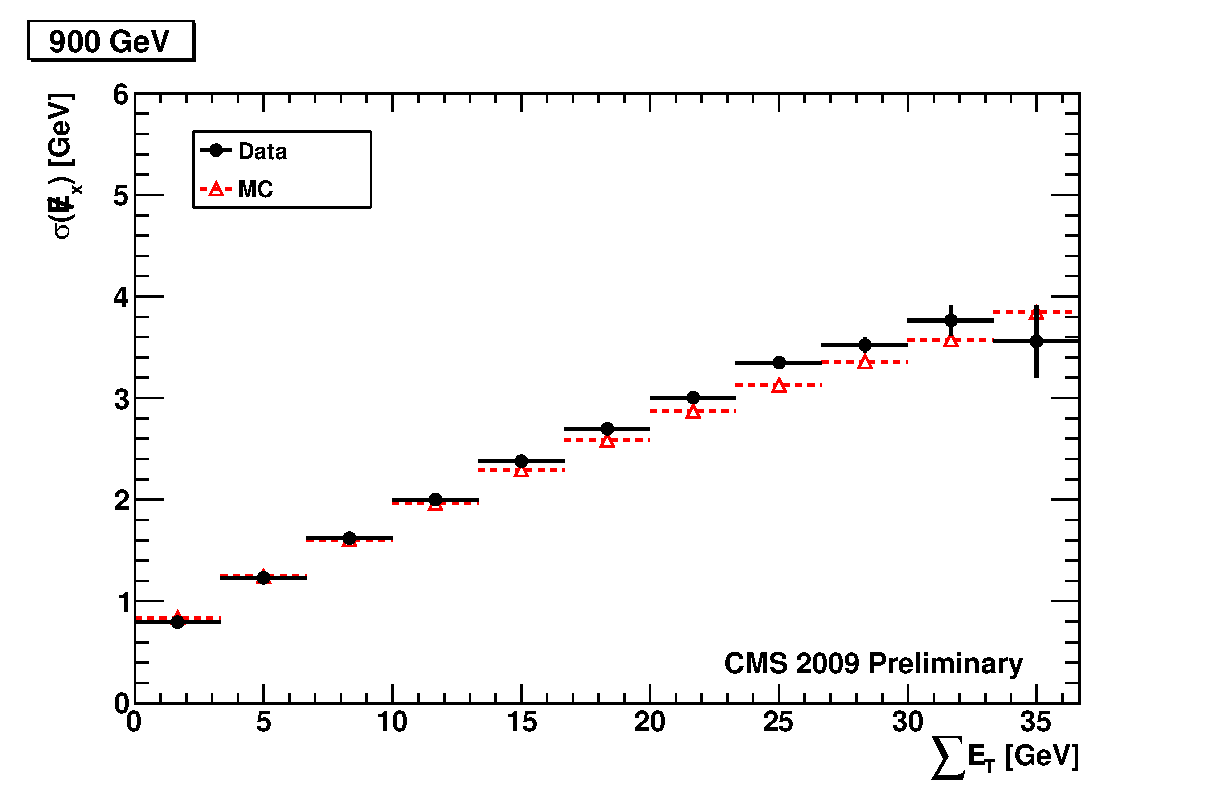
\includegraphics[width=0.5\textwidth]{plots_DataVsMC_MB_900GeV/h_metxsigma_sumet_900.eps} &
  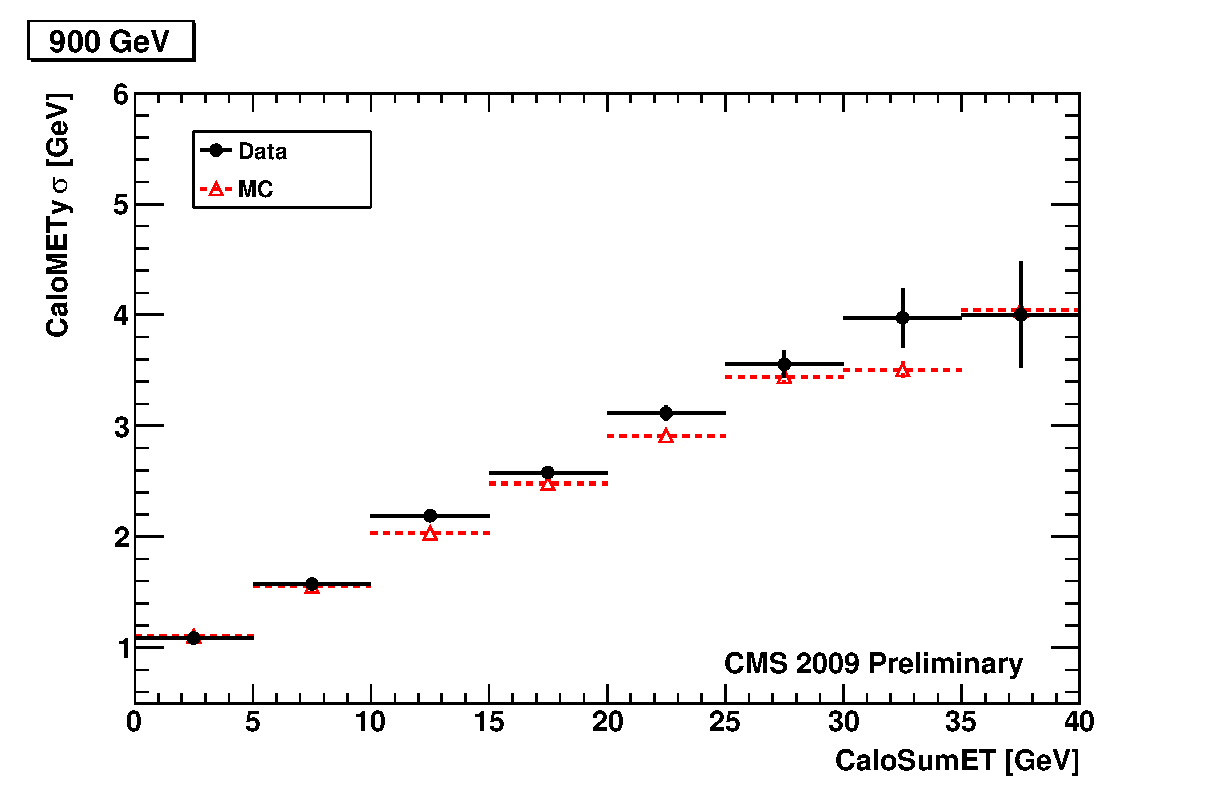
\includegraphics[width=0.5\textwidth]{plots_DataVsMC_MB_900GeV/h_metysigma_sumet_900.eps} \\
 \end{tabular}
 \caption{\small Comparison of the $\exmiss$ $\sigma$ vs. $\sum E_\text{T}$ and $\eymiss$ $\sigma$ vs. $\sum E_\text{T}$ between 
          Monte Carlo and data at $900$ GeV.\label{fig:MExySigma_vs_SumET_900}}
\end{figure}

\begin{figure}[h!]
 \centering
 \begin{tabular}{ll}
  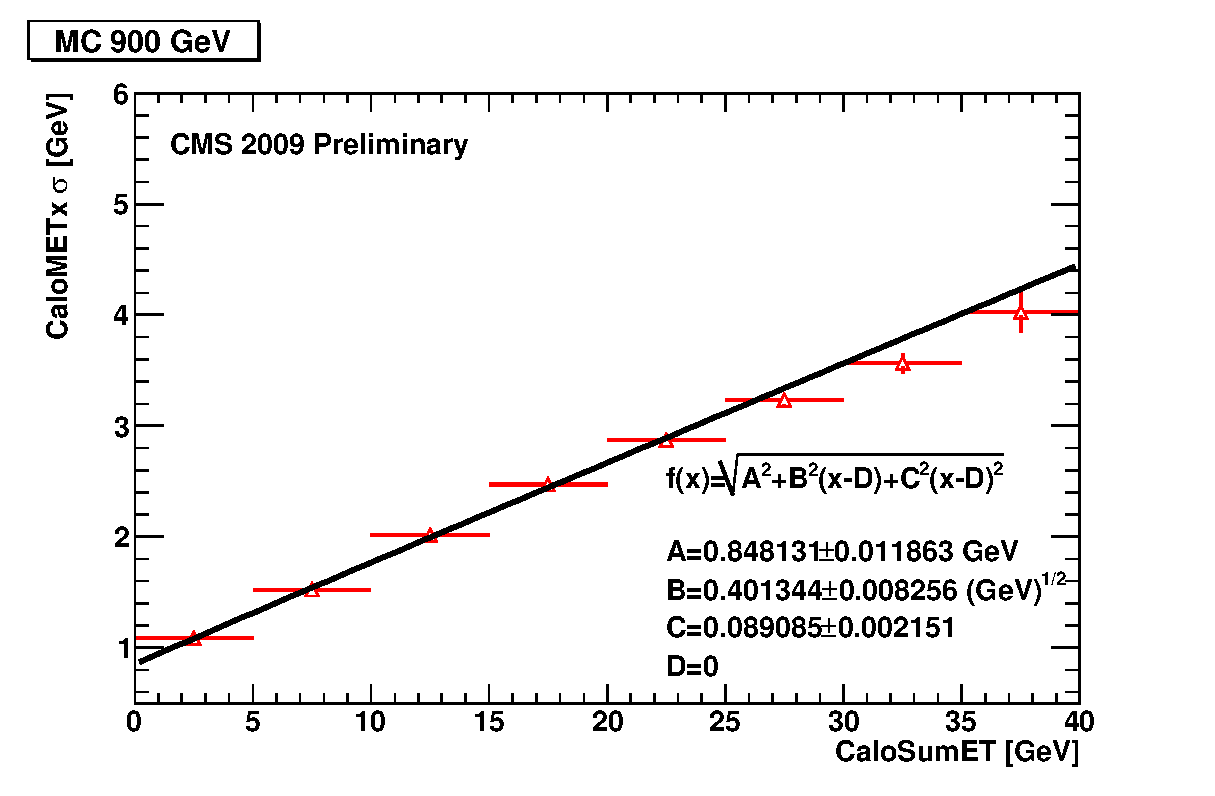
\includegraphics[width=0.5\textwidth]{plots_DataVsMC_MB_900GeV/final_metxsigma_sumet_MC_900.eps} &
  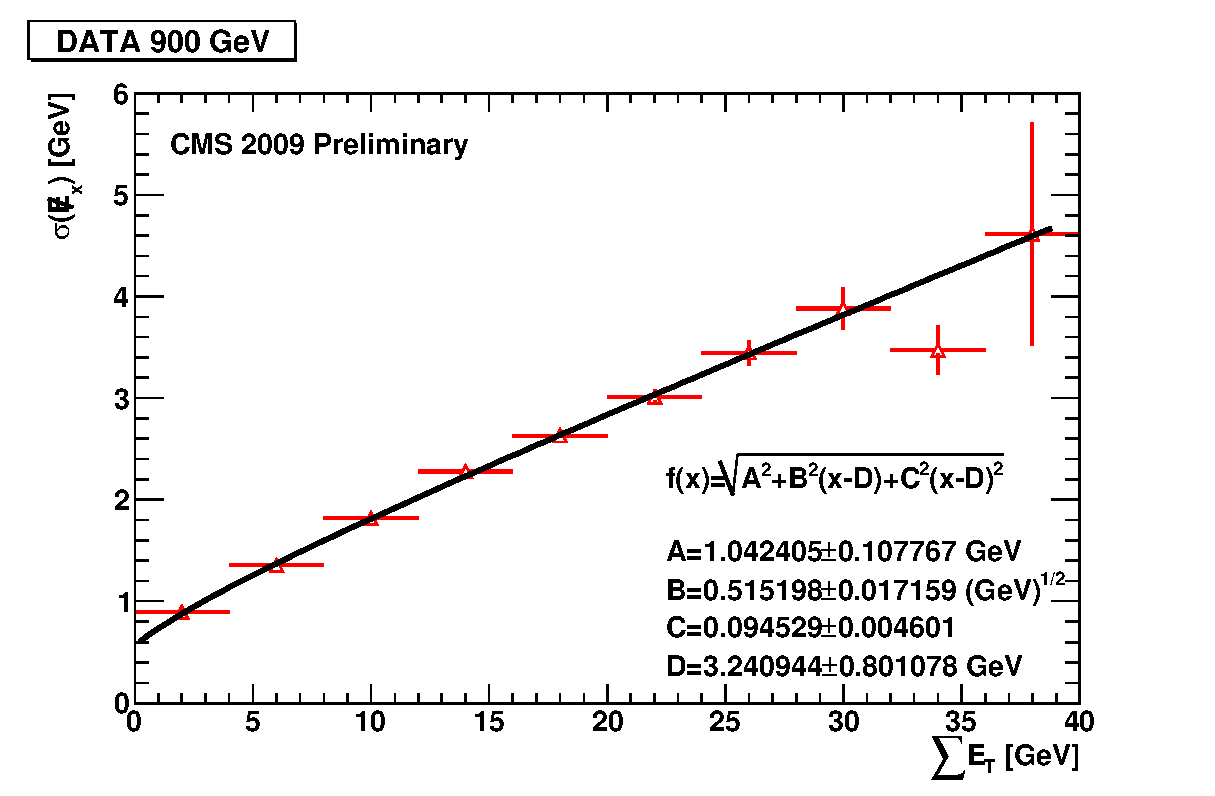
\includegraphics[width=0.5\textwidth]{plots_DataVsMC_MB_900GeV/final_metxsigma_sumet_DATA_900.eps} \\
 \end{tabular}
 \caption{\small Fit of the $\exmiss$ $\sigma$ vs. $\sum E_\text{T}$ for Monte Carlo and data at $900$ GeV. Parameter $D$ in the fit was fixed
          to zero.\label{fig:MExSigma_vs_SumET_900_fit}}
\end{figure}

\begin{figure}[h!]
 \centering
 \begin{tabular}{ll}
  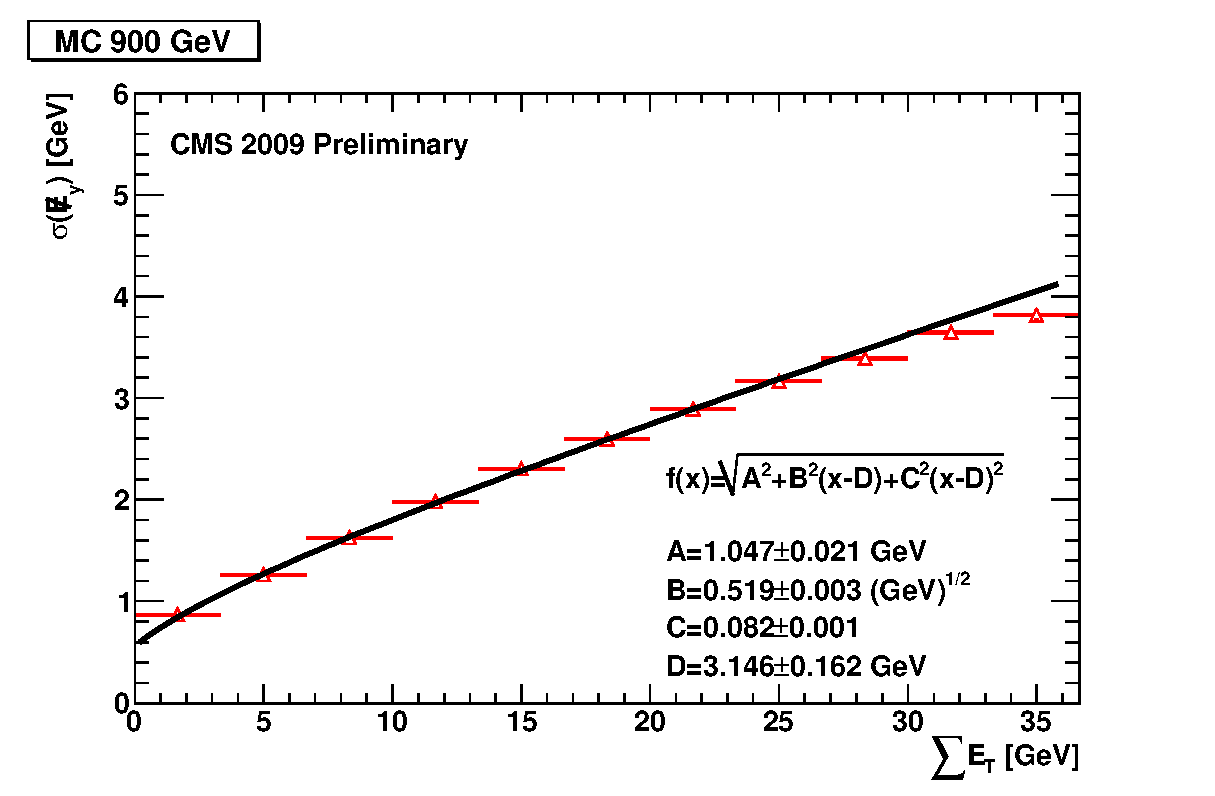
\includegraphics[width=0.5\textwidth]{plots_DataVsMC_MB_900GeV/final_metysigma_sumet_MC_900.eps} &
  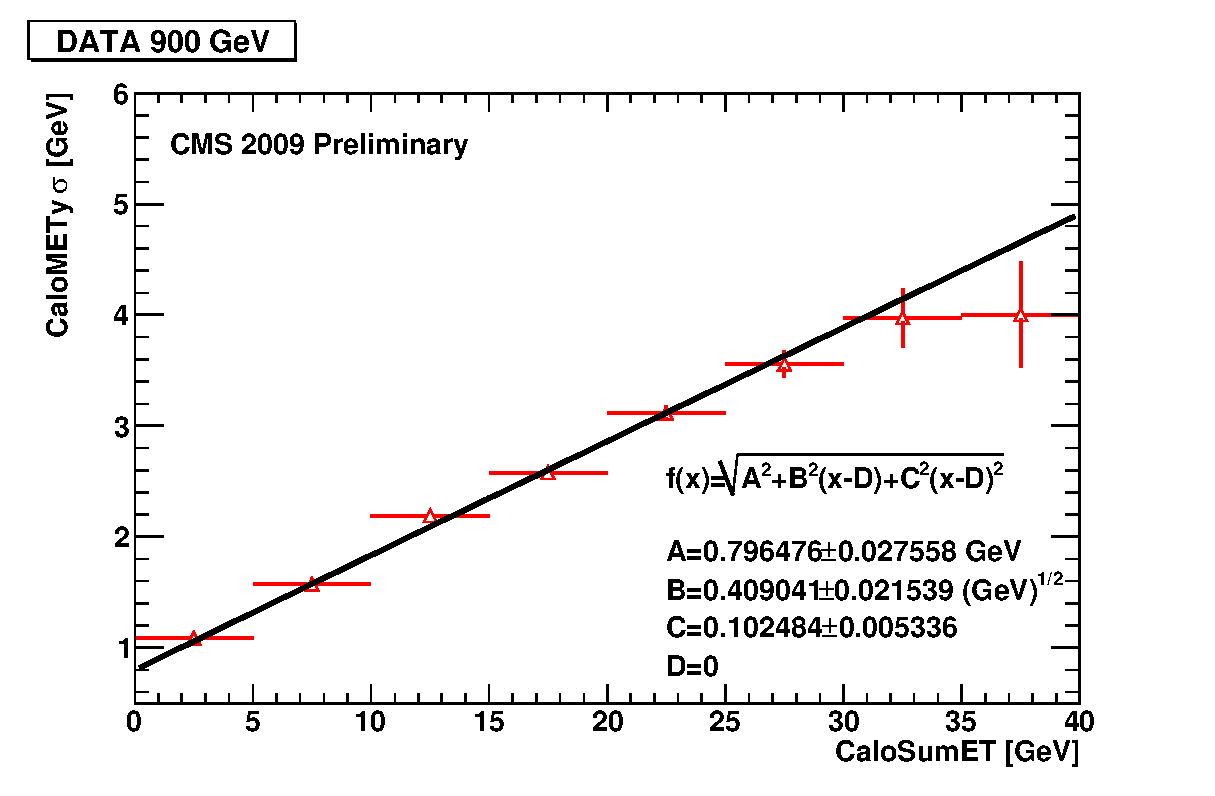
\includegraphics[width=0.5\textwidth]{plots_DataVsMC_MB_900GeV/final_metysigma_sumet_DATA_900.eps} \\
 \end{tabular}
 \caption{\small Fit of the $\eymiss$ $\sigma$ vs. $\sum E_\text{T}$ for Monte Carlo and data at $900$ GeV. Parameter $D$ in the fit was fixed
          to zero.\label{fig:MExSigma_vs_SumET_900_fit}}
\end{figure}

\clearpage

\subsection{$\etmiss$ and SumET dependence on $\eta$}

\begin{figure}[h!]
 \centering
 \begin{tabular}{ll}
  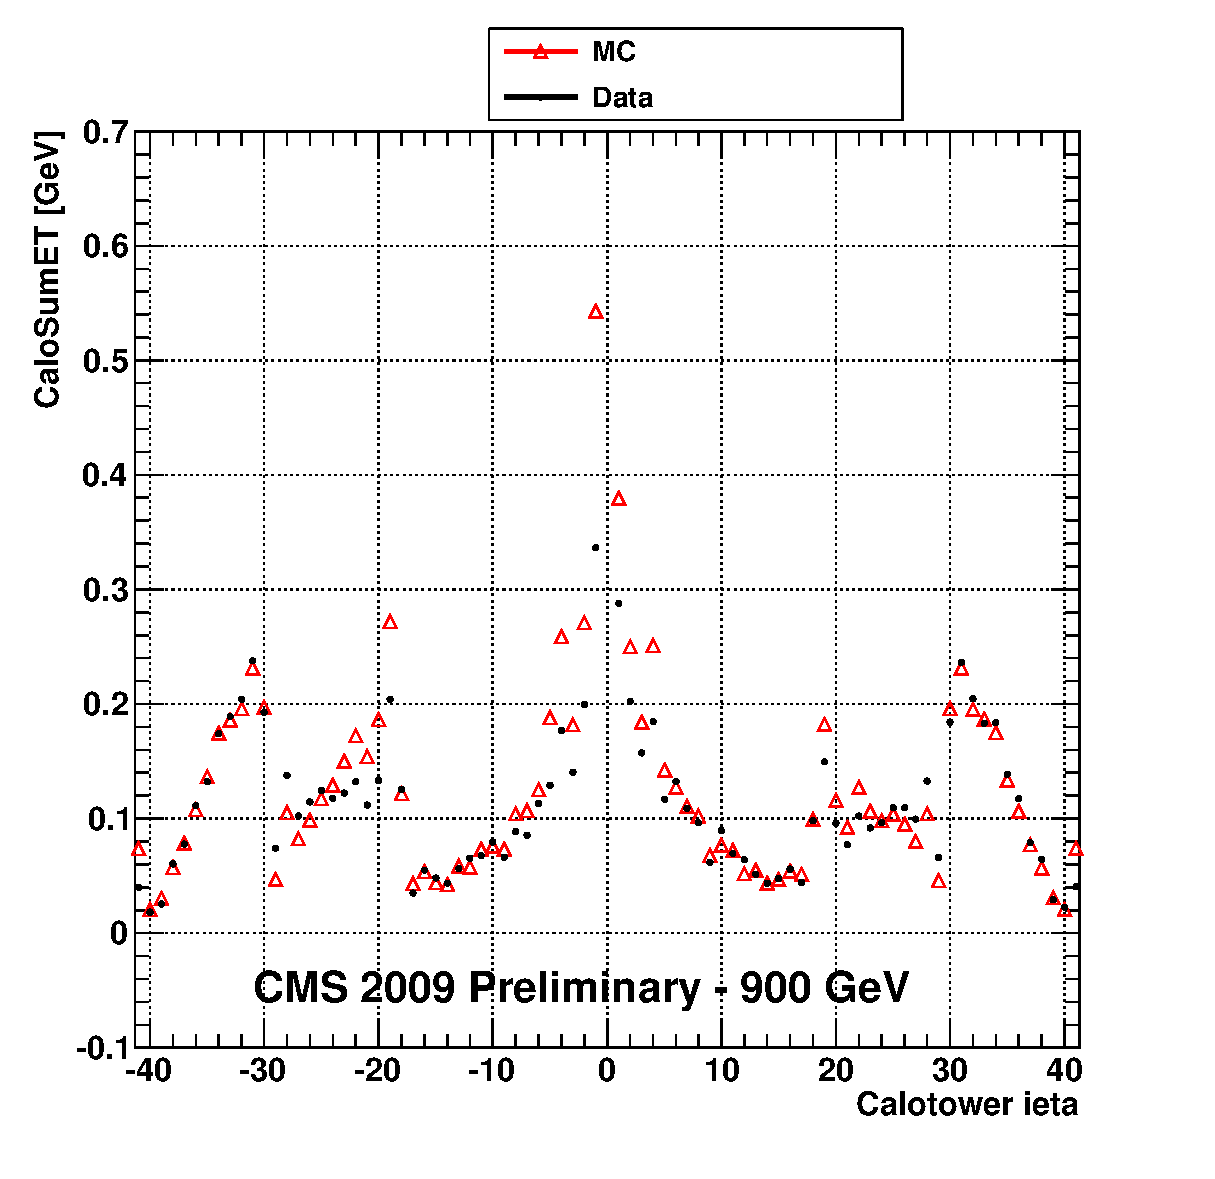
\includegraphics[width=0.5\textwidth]{plots_DataVsMC_MB_900GeV/g_caloSumetMean_vs_ieta_900.eps} &
  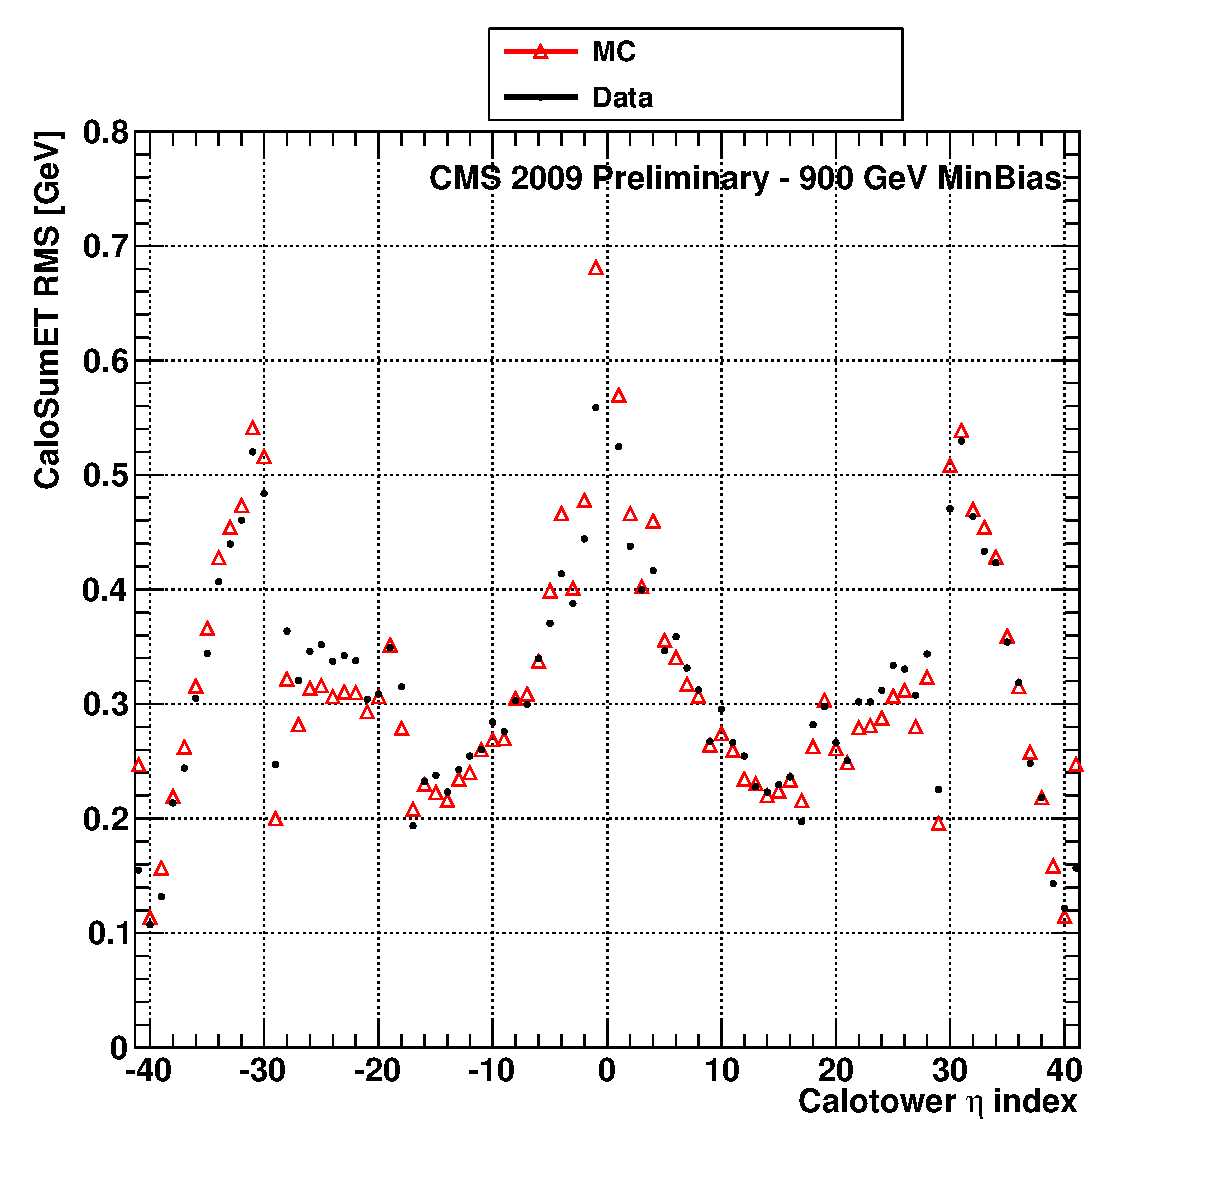
\includegraphics[width=0.5\textwidth]{plots_DataVsMC_MB_900GeV/g_caloSumetRMS_vs_ieta_900.eps} \\
 \end{tabular}
 \caption{\small Comparison of the SumET Mean vs. i$\eta$ of calotowers and SumET RMS vs. i$\eta$ of calotowers between 
          Monte Carlo and data at $900$ GeV.\label{fig:SumET_MeanRMS_vs_ieta_900}}
\end{figure}

\begin{figure}[h!]
 \centering
 \begin{tabular}{ll}
  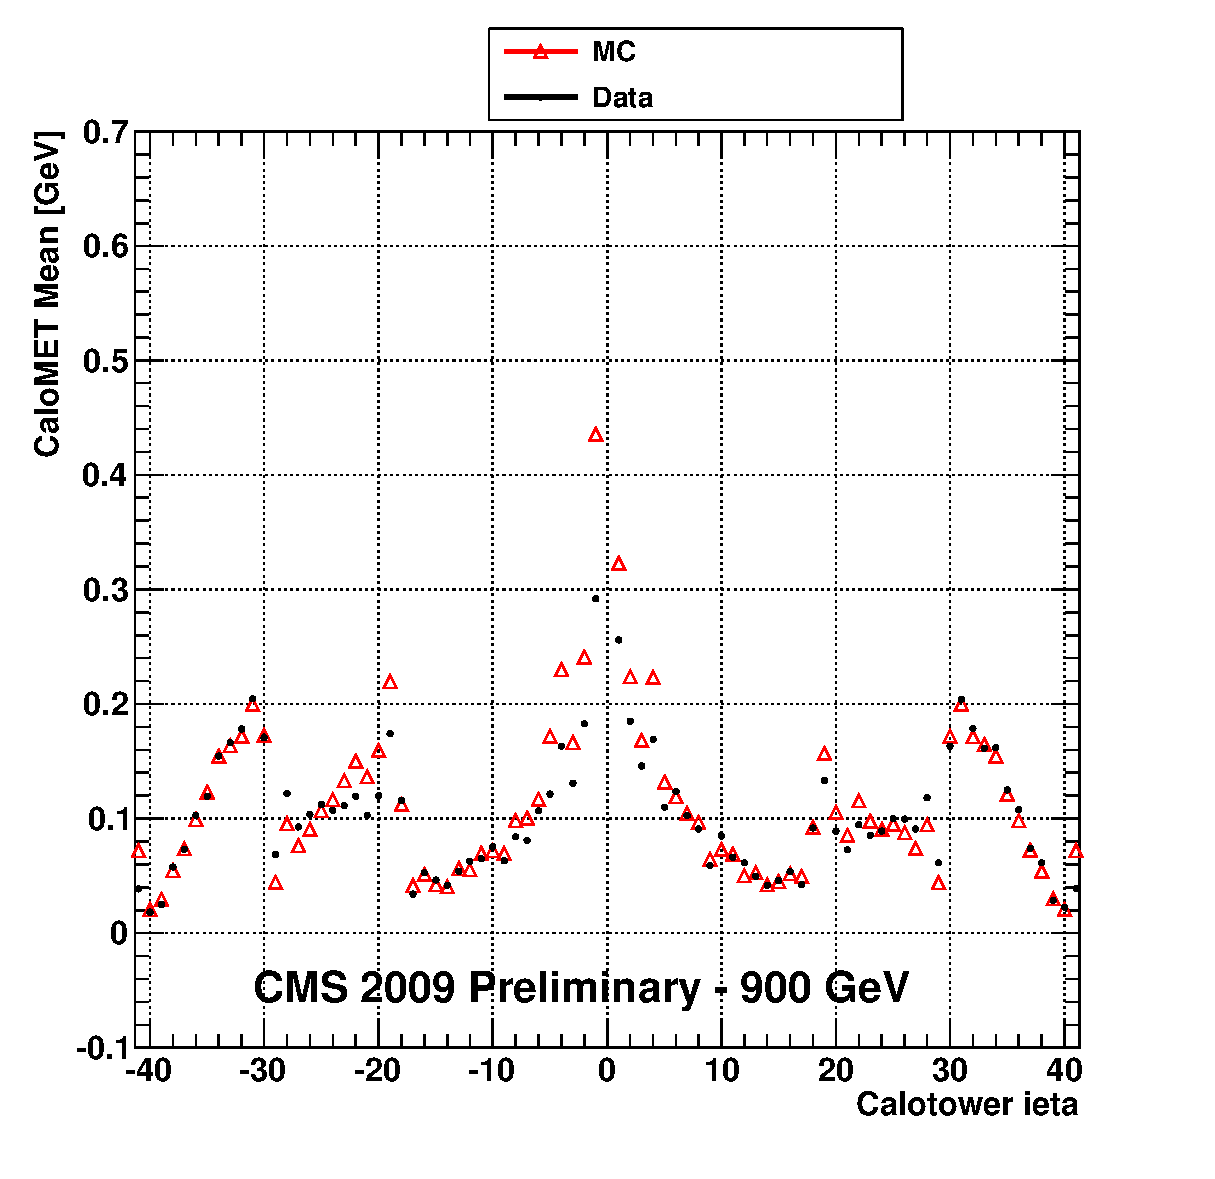
\includegraphics[width=0.5\textwidth]{plots_DataVsMC_MB_900GeV/g_calometPtMean_vs_ieta_900.eps} &
  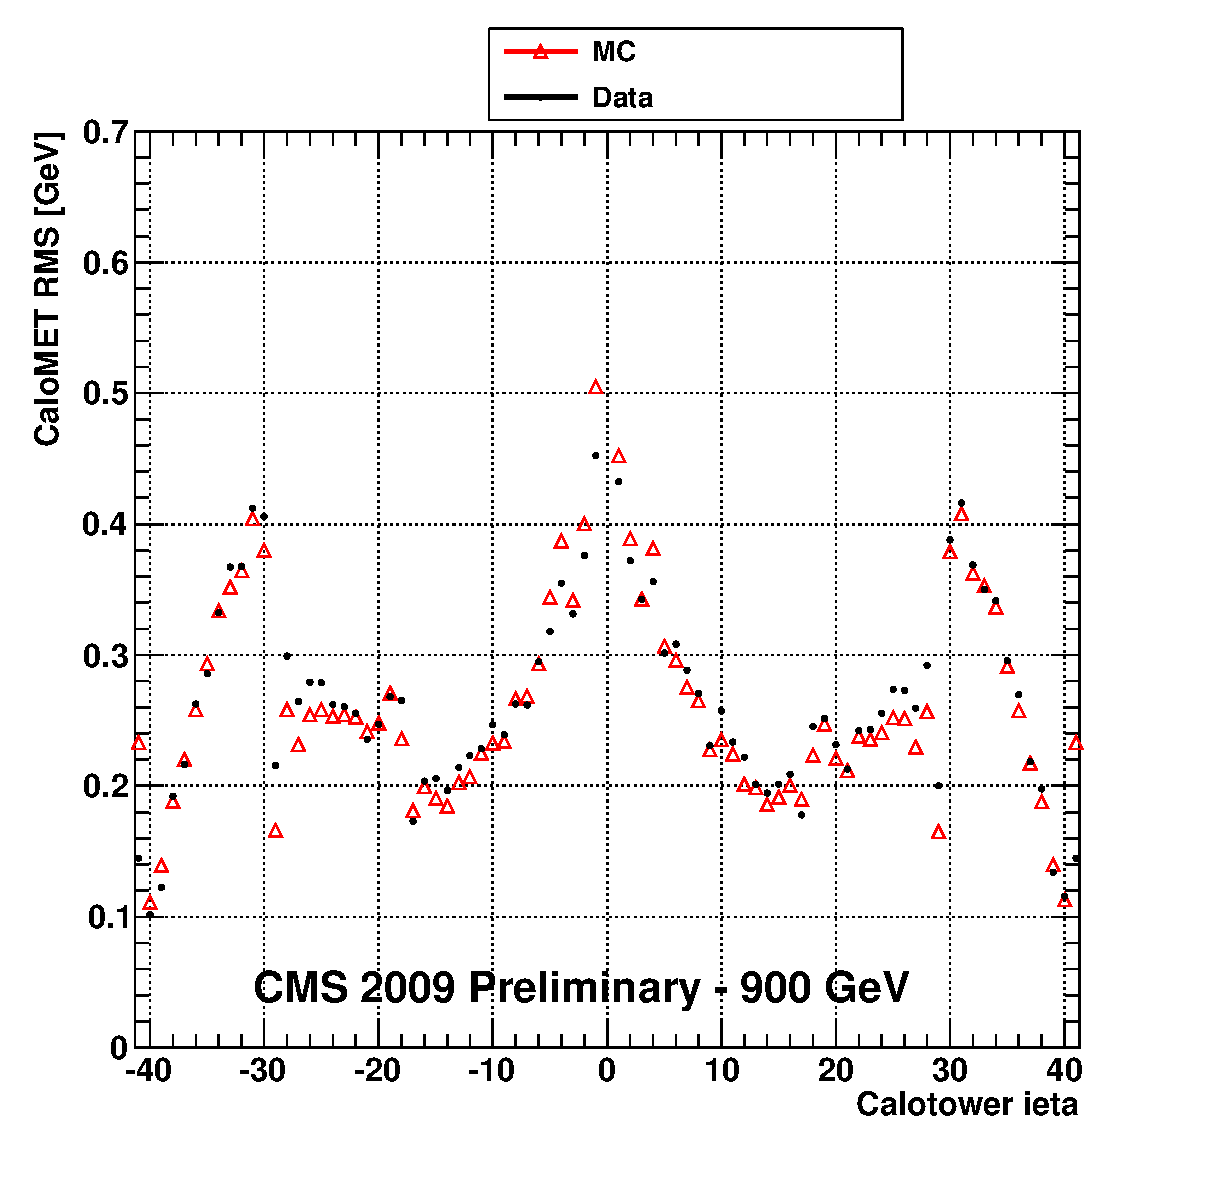
\includegraphics[width=0.5\textwidth]{plots_DataVsMC_MB_900GeV/g_calometPtRMS_vs_ieta_900.eps} \\
 \end{tabular}
 \caption{\small Comparison of the $\etmiss$ Mean vs. i$\eta$ of calotowers and $\etmiss$ RMS vs. i$\eta$ of calotowers between 
          Monte Carlo and data at $900$ GeV.\label{fig:MET_MeanRMS_vs_ieta_900}}
\end{figure}

\begin{figure}[h!]
 \centering
 \begin{tabular}{ll}
  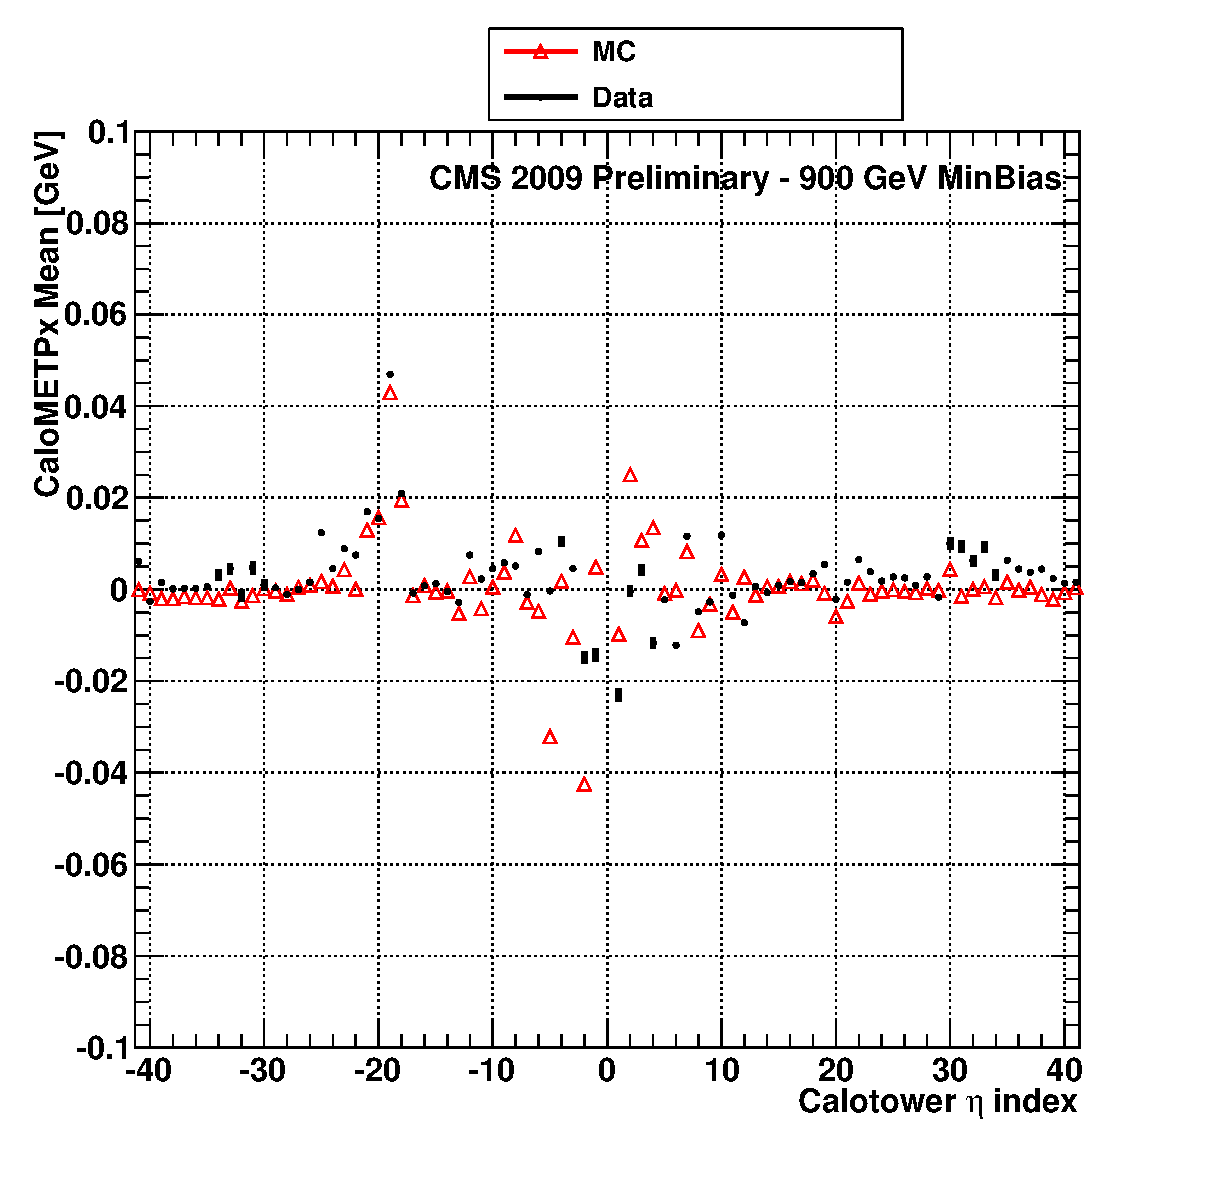
\includegraphics[width=0.5\textwidth]{plots_DataVsMC_MB_900GeV/g_calometPxMean_vs_ieta_900.eps} &
  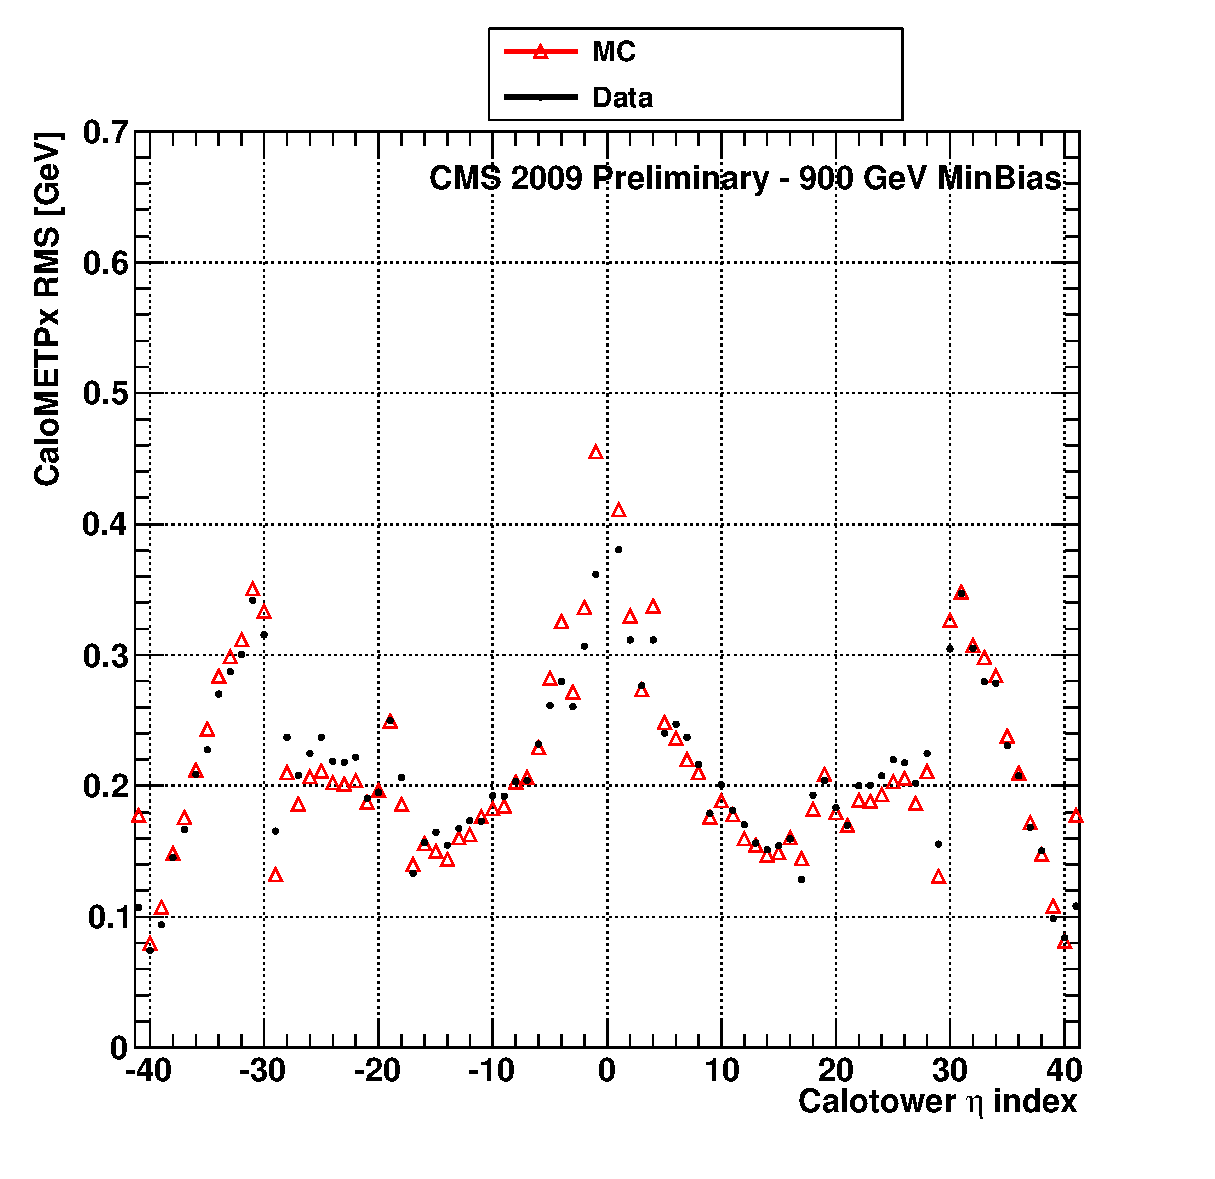
\includegraphics[width=0.5\textwidth]{plots_DataVsMC_MB_900GeV/g_calometPxRMS_vs_ieta_900.eps} \\
 \end{tabular}
 \caption{\small Comparison of the $\exmiss$ Mean vs. i$\eta$ of calotowers and $\exmiss$ RMS vs. i$\eta$ of calotowers between 
          Monte Carlo and data at $900$ GeV.\label{fig:METx_MeanRMS_vs_ieta_900}}
\end{figure}

\begin{figure}[h!]
 \centering
 \begin{tabular}{ll}
  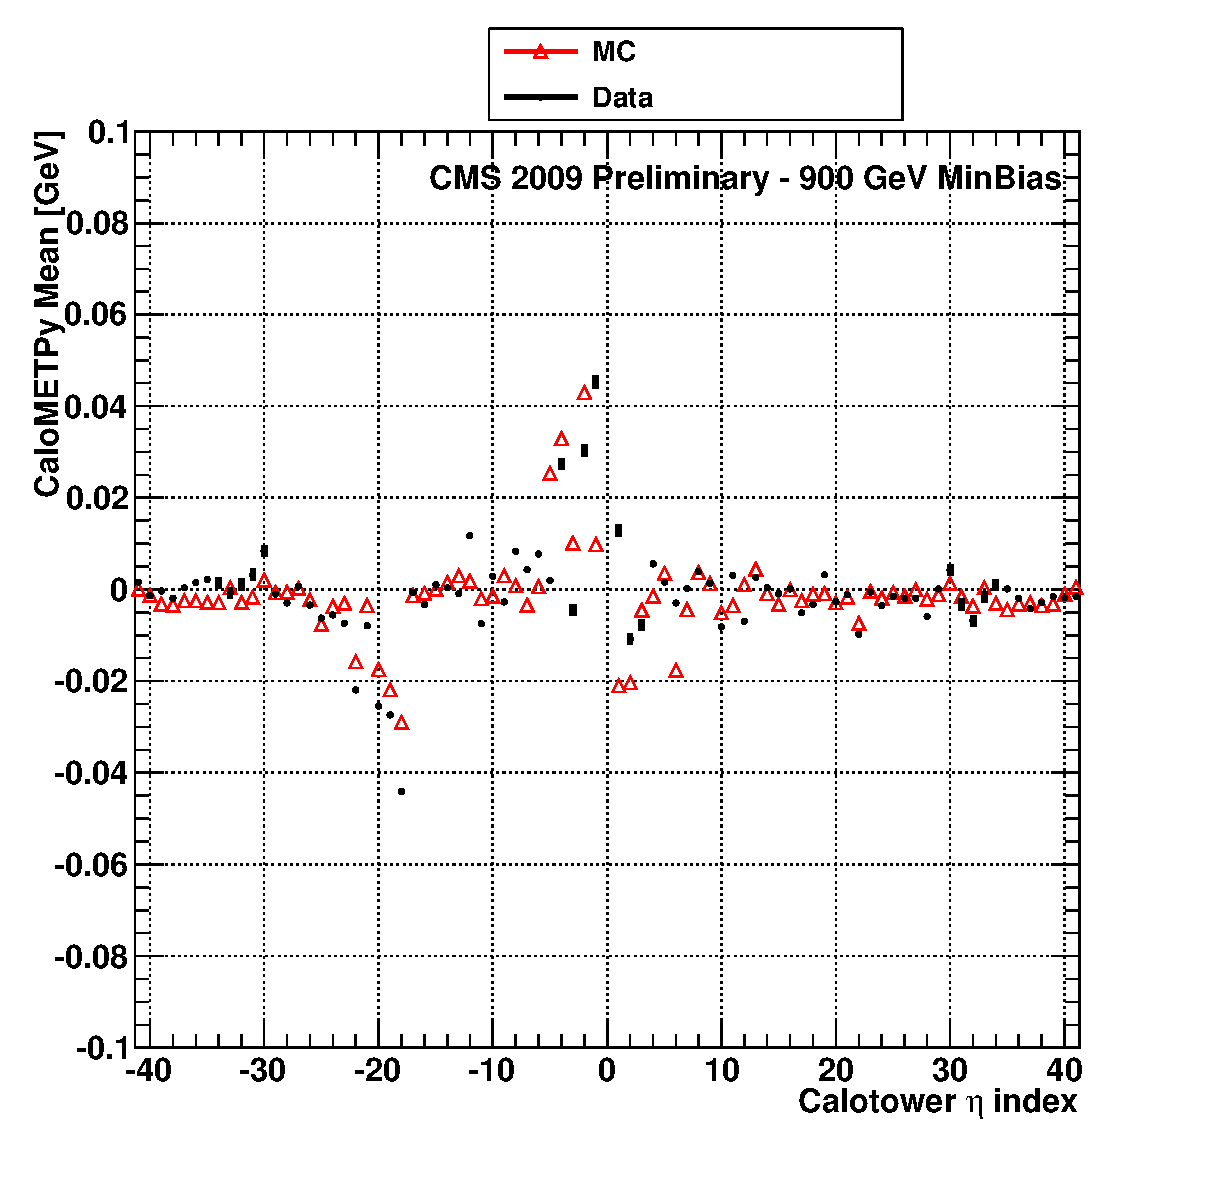
\includegraphics[width=0.5\textwidth]{plots_DataVsMC_MB_900GeV/g_calometPyMean_vs_ieta_900.eps} &
  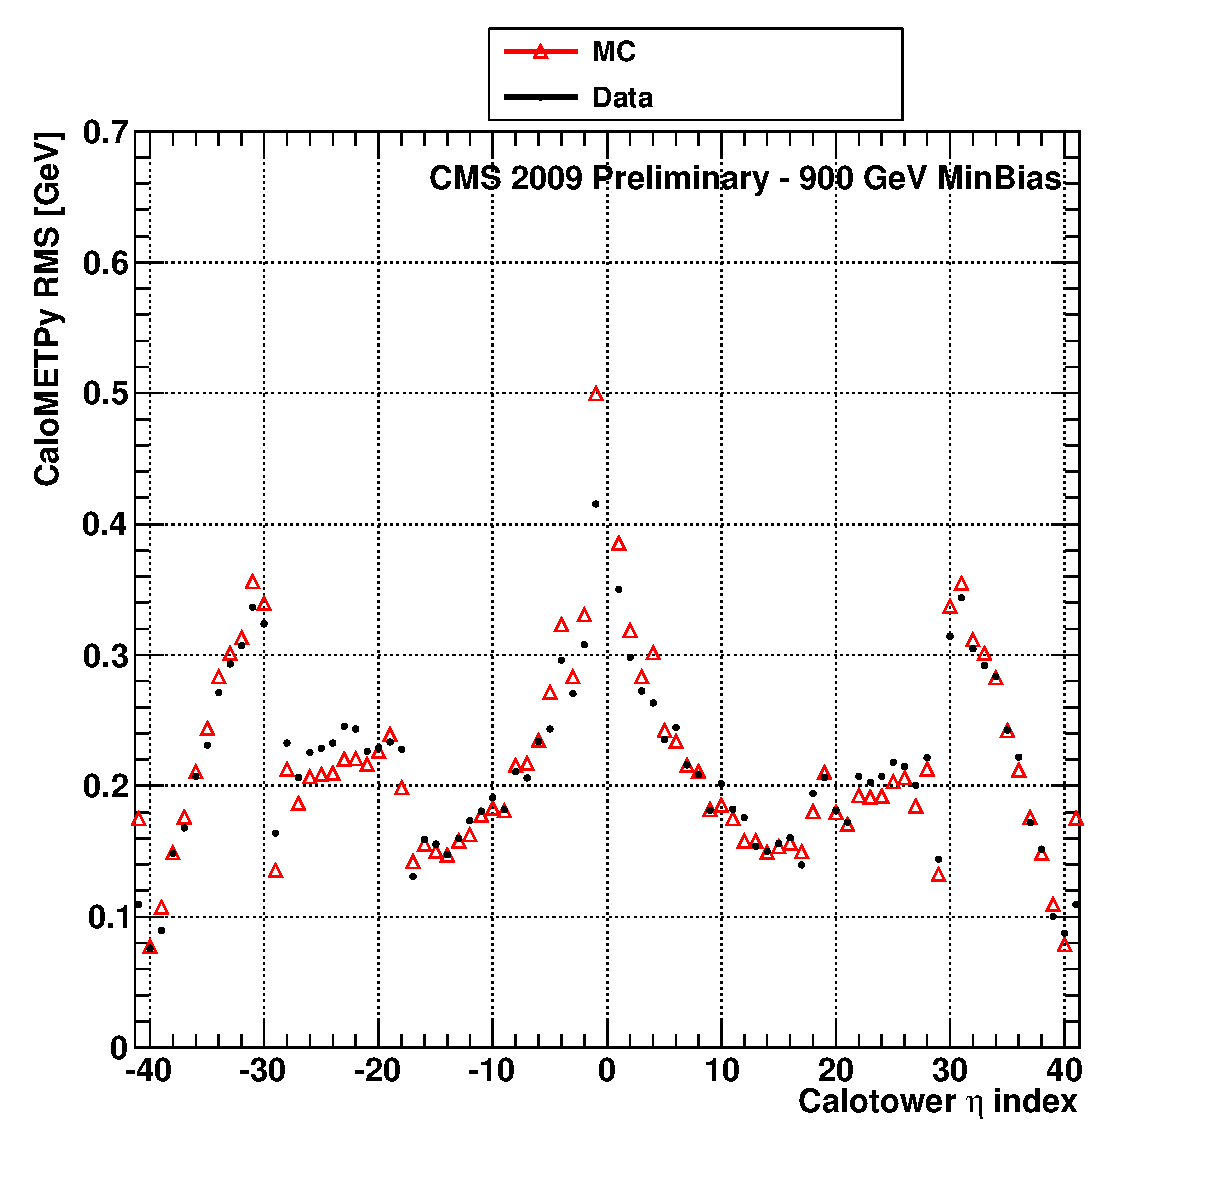
\includegraphics[width=0.5\textwidth]{plots_DataVsMC_MB_900GeV/g_calometPyRMS_vs_ieta_900.eps} \\
 \end{tabular}
 \caption{\small Comparison of the $\eymiss$ Mean vs. i$\eta$ of calotowers and $\eymiss$ RMS vs. i$\eta$ of calotowers between 
          Monte Carlo and data at $900$ GeV.\label{fig:METy_MeanRMS_vs_ieta_900}}
\end{figure}

\clearpage
